\documentclass{sig-alternate}

\usepackage[
hidelinks,
pdftitle={Cognitive Disconnect: Understanding Facebook Connect Login Permissions},
pdfauthor={Nicky Robinson and Joseph Bonneau}
]{hyperref}
\usepackage[usenames,dvipsnames]{xcolor}
\usepackage{multirow}
\usepackage{graphicx}
\usepackage{float}
\usepackage{subfloat}
\usepackage{caption}
\usepackage{placeins}
\usepackage{verbatim}

\setlength{\paperheight}{11in}
\setlength{\paperwidth}{8.5in}
\usepackage[
  pass,% keep layout unchanged 
  % showframe,% show the layout
]{geometry}

\let\proof\relax
\let\endproof\relax
\usepackage{amsthm}

\newtheorem{hypothesis}{Null Hypothesis}

%\newcommand{\extendedversion}[2]{#1}
\newcommand{\extendedversion}[2]{#2}


% copyright notice
\newfont{\mycrnotice}{ptmr8t at 7pt}
\newfont{\myconfname}{ptmri8t at 7pt}
\let\crnotice\mycrnotice%
\let\confname\myconfname%

\permission{Permission to make digital or hard copies of all or part of this work for personal or classroom use is granted without fee provided that copies are not made or distributed for profit or commercial advantage and that copies bear this notice and the full citation on the first page. Copyrights for components of this work owned by others than ACM must be honored. Abstracting with credit is permitted. To copy otherwise, or republish, to post on servers or to redistribute to lists, requires prior specific permission and/or a fee. Request permissions from permissions@acm.org.}
\conferenceinfo{COSN'14,}{October 1--2, 2014, Dublin, Ireland.}
\copyrightetc{Copyright 2014 ACM \the\acmcopyr}
\crdata{978-1-4503-3198-2/14/10\ ...\$15.00.\\
http://dx.doi.org/10.1145/2660460.2660471}
\clubpenalty=10000
\widowpenalty = 10000


\begin{document}\sloppy

\definecolor{darkred}{HTML}{E50000}

\title{Cognitive Disconnect:\\ Understanding Facebook Connect Login Permissions}

\numberofauthors{2} 
\author{
\alignauthor
Nicky Robinson\\
       \affaddr{Princeton University}\\
       \email{ncrobins@princeton.edu}
\alignauthor
Joseph Bonneau\\
       \affaddr{Princeton University}\\
       \email{jbonneau@princeton.edu}
}

\maketitle

\begin{abstract}
We study Facebook Connect's permissions system using crawling, experimentation, and user surveys.
We find several areas in which it it works differently than many users and developers expect.
More permissions can be granted than developers intend.
In particular, permissions that allow a site to post to the user's profile are granted on an all-or-nothing basis.
%We evaluate how the requested permissions are presented to the user and find that.
While users generally understand what data sites can read from their profile, they generally do not understand the full extent of what sites can post.
In the case of write permissions, we show that user expectations are influenced by the identity of the requesting site although this has no impact on what is actually enforced.
We also find that users generally do not understand the way Facebook Connect permissions interact with Facebook's privacy settings.
Our results suggest that users understand detailed, granular messages better than those that are broad and vague.
%In order to protect users' privacy, Facebook should granularize the write permissions, present them to the user more distinctly, and make clear the way privacy settings are handled.

% sentence about what the takeaway is. should fb do something? should users be more vigilent?

% should we mention federated identity
\end{abstract}

\category{D.4.6}{Security and Protection}{Access Controls}
\terms{Security; Human Factors}
\keywords{Online social networks; permissions; privacy; Facebook}

\section{Introduction}
Single Sign-On (SSO) systems allow users to log in to websites (called \textit{relying sites} or \textit{relying parties}) using their username and password from a third-party \textit{identity provider}.
This creates fewer passwords for users to remember, theoretically meaning that they can have more complicated and therefore more secure passwords \cite{openidsecurity}.
Facebook Connect\footnote{Facebook Connect is now technically called Facebook Login but is still frequently referred to as Facebook Connect.} is perhaps the most popular SSO system on the web today.
A key reason is that Facebook Connect, like many SSO systems based off of the OAuth protocol, does more than just allow a user to sign in: sites can request access to read parts of the user's Facebook profile or write data back their profile.
This has been sufficient in practice to overcome the lack of adoption incentives for relying parties which has plagued many other SSO systems on the web~\cite{sun10}.
%This is a feature of many SSO systems based off of the OAuth protocol.

An important selling point is that Facebook Connect requires relying sites to request a specific set of permissions from the user up front in order to read or write data from the user's profile.
These are presented to the user in a series of dialogues (shown in Figure~\ref{figure:messageexample}) which the user must approve prior to logging into a relying site for the first time.
In the words of Facebook, \textit{``The user will have total control of the permissions granted''}~\cite{fb-connect-announce}.
%Facebook Login requires user approval Developers integrating Facebook Connect may request various permissions from Facebook allowing them to see information on the user's profile or publish content to their profile. %The permissions available to the developer can be seen in the Facebook Connect documentation \cite{fbpermissions}.

%probably too much for the intro
\begin{comment}
When a user logs in to a website using Facebook Connect, they are presented with up to three dialogues asking them to authorize the website to receive the desired permissions. The first message corresponds to the \emph{read} permissions, permissions that allow the site to see information on the user's profile. The second corresponds to the \emph{write} permissions, which allow the site to post various things on the user's profile. The third (or second, if no write permissions were requested) corresponds to the \emph{extended} permissions. These permissions are for more sensitive things, such as sending the user text messages and marking their notifications as read. The user can refuse to grant write and extended permissions and still log in.\footnote{The documentation \cite{fbpermsinstructions} provides more details about these groups, although it breaks them down into six different groups.} If the user approves these permissions, they are logged in to the site and the site receives their information from Facebook.  shows examples of messages asking the user to authorize permissions.
\end{comment}

%Users logging in with Facebook Connect place a lot of trust in Facebook to only share information that the user authorizes.
Effective user control relies both on Facebook granting only the permissions intended by developers and on users correctly understanding the permissions they approve.
We explore both assumptions and show that:

\begin{figure*}[htbp]
  \centering
  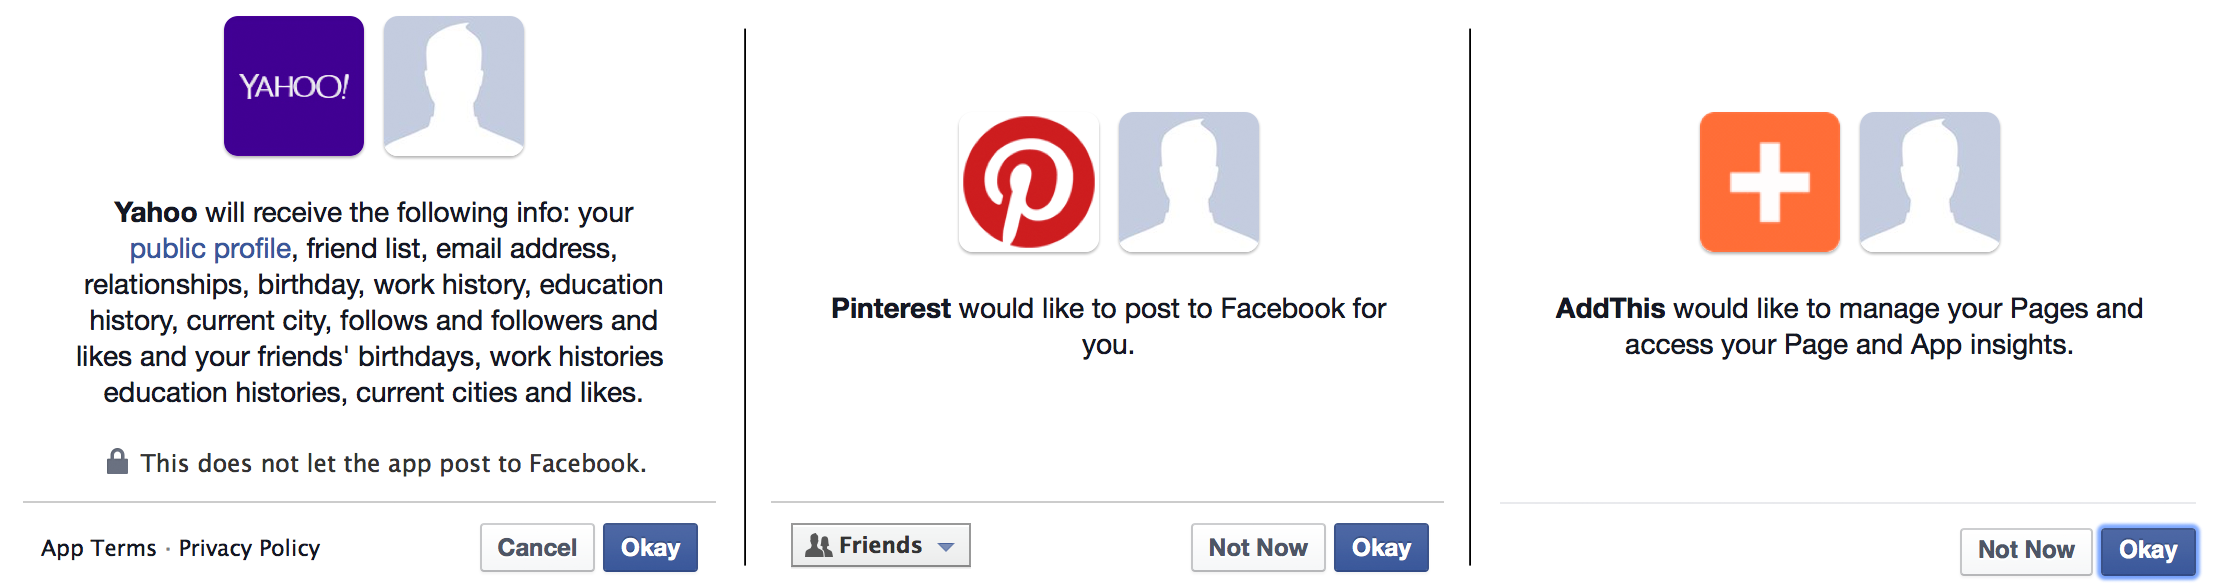
\includegraphics[width=16.5cm]{message_example}
  \caption{Examples of messages presented to the user. From left: Read permissions message from Yahoo.com, write permissions message from Pinterest.com, and extended permissions message from AddThis.com.}
  \label{figure:messageexample}
\end{figure*}

\begin{itemize}
  \item Facebook Connect sometimes asks the user to authorize more permissions than the developer intended to request.
  \item Write permissions are granted to sites on an all-or-nothing basis. For example, if a site wants the ability to update the user's status, it must also gain the ability to upload photos.
  \item Users generally understand which read permissions are being requested when they log in, although many do not realize they are granting access to data they have marked as private using their privacy settings.
  \item Users generally do not understand the variety of write permissions sites will receive upon authorization. This indicates that, despite Facebook's claim that all-or-nothing write permissions are ``simpler'' for users to understand, users understand the more granular read permissions better.
  \item  Users are influenced by the identity of the relying site; for example, they are much more likely to understand a photo sharing website can upload photos to their account. This suggests users are assuming a \textit{contextual integrity} model of privacy~\cite{contextual-integrity}, although this is not implemented technically.
\end{itemize}

\section{Implementation of Facebook Connect permissions}
\label{sec:implementation}
The first step in determining whether the permissions system provides users with effective control is understanding which permissions are actually granted when a given authorization message is displayed.
Facebook Connect's process of a site requesting permissions from a user can be broken down into three steps:

\begin{enumerate}
  \item During login flow, relying parties request a set of permissions from the Facebook Connect API. We'll call this set the \textit{requested permissions}.
  \item Facebook receives the requested permissions and translates them into a set of permissions for approval which we'll call the \textit{granted permissions}.
  \item Facebook translates the the granted permissions into a dialogue presented to the user for approval. We'll call this text the \textit{displayed permissions}.
\end{enumerate}

Ideally, these three sets of permissions would be semantically identical and the text shown to the user would clearly represent them. In this section we'll explore the difference between the requested and granted permissions; we'll compare displayed and granted permissions in Section~\ref{sec:understanding}.

\subsection{Methodology}

Unfortunately, Facebook's documentation \cite{fbdocs} is incomplete and sometimes outdated. 
As such, there is very little explanation of how requested permissions are eventually translated into permissions displayed to the user.
To gain a better understanding, we combined information from the documentation with observations from integrating Facebook Connect login with a test site and crawled data from several hundred relying sites.

\subsubsection{Obtaining a list of relying sites}

%The data from real sites was obtained by web crawling. The first step was to compile a list of sites with Facebook Connect logins.
To obtain a list of relying sites implementing Facebook Connect, we started with the most recent (October 2013) AppInspect \cite{appinspect} database of 25,000 Facebook apps.
We filtered this list down to about 400 apps with an external site listed on the Facebook App Center.
Finally, we manually idenitified 91 which had a Facebook Connect login.

Unfortunately, the AppInspect database does not include apps that are used solely for Facebook Connect, only those that have native Facebook apps. 
%In part because of this, the majority of the sites we found from the database are relatively obscure.
To make up for these deficiencies, we took the Alexa Top 500\footnote{\url{http://www.alexa.com/topsites}} websites from February 27\textsuperscript{th}, 2014 and manually identified those with Facebook Connect logins (112 sites). 
Combining these two lists gave us a total of 203 sites to study.
%, about half which receive heavy traffic (those from the Alexa Top 500) and about half of which do not (those from the AppInspect database).
%This list provides a diverse sampling of the websites people log in to with Facebook Connect.

For crawling we used OpenWPM,\footnote{\url{https://github.com/citp/OpenWPM/wiki}} a Selenium-based\footnote{\url{https://github.com/cmwslw/selenium-crawler}} web crawler being developed by the Princeton Center for Information Technology Policy (CITP). 
We performed automated logins to all 203 sites and recorded the requested, granted, and displayed permissions.
% they request and the corresponding messages presented to the users. (The way the permissions they request was determined will be discussed in Section~\ref{sec:inputels}.)
26 of the 203 sites used an older version of Facebook Connect; we will focus only on the 177 using the current version.

\subsection{Requested permissions}

%The first step in the permissions presentation process as we outlined it above is the developer designing their site to request permissions from Facebook.
Developers request permissions in a parameter called ``scope'' or ``data-scope'' when the login process is initiated using Facebook's JavaScript SDK, Facebook's login button, or a manually built login system \cite{fbpermsinstructions}.
The developer can request any of the permissions listed in the documentation \cite{fbpermissions}, although some are deprecated and will have no impact on the granted permissions.% (including, it appears, some that are not listed as deprecated).

The scope parameter is visible in the URL of the page where the user is asked to approve permissions (see Figure~\ref{figure:scopeinurl}).
We confirmed using our test site that this value is indeed exactly what the developer requested.
%When crawling the sites, we parsed the URLs to extract the permissions requested by developers.

%\floatstyle{boxed}
\restylefloat{figure}
\begin{figure}[tb!]
  {\small{\fontfamily{phv}\selectfont %https://www.facebook.com/dialogue/oauth?app\_id=138615416238413\\\&client\_id=138615416238413\&display=popup\&domain=www.timecr\\unch.me\&e2e=\%7B\%7D\&locale=en\_US\&origin=1\&redirect\_uri=http\\\%3A\%2F\%2Fstatic.ak.facebook.com\%2Fconnect\%2Fxd\_arbiter\%2\\F8n77RrR4jg0.js\%3Fversion\%3D40\%23cb\%3Df17cdd7f881aff\%26\\domain\%3Dwww.timecrunch.me\%26origin\%3Dhttp\%253A\%252F\%\\252Fwww.timecrunch.me\%252Ff2dc123d3ff5394\%26relation\%3Do\\pener\%26frame\%3Df25cadbc2ca73cc\&response\_type=token\%2Csi\\gned\_request\&{\color{darkred}scope=email\%2Ccreate\_event\%2Coffline\_access\%2\\Cuser\_groups\%2Cfriends\_groups\%2Cpublish\_stream}\&sdk=joey}}
https://www.facebook.com/dialogue/oauth?app\_id=138615416238413\\
\&domain=www.timecrunch.me\&response\_type=token\%2Csigned\_re\\
quest\&{\color{darkred}scope=email\%2Ccreate\_event\%2Coffline\_access\%2Cuser\_gr\\
oups\%2Cfriends\_groups\%2Cpublish\_stream}...}}
\caption{Example requested permissions (colored in red) in the scope parameter of the approval page URL.
  %The permissions being requested are \emph{email}, \emph{create\_event}, \emph{offline\_access} (deprecated), \emph{user\_groups}, \emph{friends\_groups}, and \emph{publish\_stream}. (`\%2C' represents a comma.)
  }
  \label{figure:scopeinurl}
\end{figure}
%\floatstyle{plain}
\restylefloat{figure}
\subsection{Granted permissions}

Facebook receives the requested permissions and translates them into a set of granted permissions. The granted permissions may exclude requested permissions that are deprecated, or, in some cases, may add additional permissions. 
%In the second step, a user visiting a site initiates the login process and Facebook creates a set of permissions that the site will get from Facebook if the user approves them. Theoretically and ideally this set would be identical to the one that the developer requested, but in practice this is not the case.
Two permissions, which Facebook calls ``Basic Info/Default permissions''\cite{fbpermsinstructions}, are always added regardless of what is requested: \emph{public\_profile} and \emph{user\_friends}. The documentation does not mention any other permissions that may be granted outside of what the developer requested.

%\subsubsection{Identifying granted permissions in practice}
\label{sec:inputels}

%The Facebook documentation does not say how a user presented with a message asking them to authorize permissions can identify the exact permissions being requested---they have only the message presented to them. But to understand how Facebook handles permissions, we need to know exactly which permissions will be granted if the user clicks okay. 

The approval page presented to the user has three hidden input HTML elements named \emph{read}, \emph{write}, and \emph{extended} whose values are the granted permissions (see Figure~\ref{figure:inputels}).
We confirmed with our test site that these permissions are actually granted and may be used by the relying site, regardless of the requested permissions.
%Further investigation indicates that these three elements hold all of the permissions that will be granted if the user clicks okay (and the scope variable in the URL does not).

\begin{figure}[tb]
  \centering
  \def\arraystretch{1.3}
  \begin{tabular}{l}
     
    {\scriptsize\fontfamily{pcr}\selectfont 
      \vtop{\hbox{\strut{<{\color{RoyalPurple}input} type=``{\color{blue}hidden}'' autocomplete=``{\color{blue}off}'' name=}}\hbox{\strut{``{\color{blue}read}'' value=``{\color{darkred}email,user\_groups,friends\_groups,}}}\hbox{\strut{{\color{darkred}public\_profile,user\_friends,private}'' />}}}
    }\\
    {\scriptsize\fontfamily{pcr}\selectfont 
      \vtop{\hbox{\strut{<{\color{RoyalPurple}input} type=``{\color{blue}hidden}'' autocomplete=``{\color{blue}off}'' name=}}\hbox{\strut{``{\color{blue}write}'' value=``{\color{darkred}publish\_stream,publish\_actions,}}}\hbox{\strut{{\color{darkred}create\_note,photo\_upload,publish\_checkins,share\_item,}}}\hbox{\strut{{\color{darkred}status\_update,video\_upload}'' />}}}
    }\\
    {\scriptsize\fontfamily{pcr}\selectfont 
      \vtop{\hbox{\strut{<{\color{RoyalPurple}input} type=``{\color{blue}hidden}'' autocomplete=``{\color{blue}off}'' name=}}\hbox{\strut{``{\color{blue}extended}'' value=``{\color{darkred}create\_event,rsvp\_event}'' />}}}
    } \\ 
  \end{tabular}
  \caption{Example granted permissions (colored in red) shown by the \emph{read}, \emph{write}, and \emph{extended} input elements on the permissions approval page for \url{timecrunch.me}. 
  %Permissions are colored red. 
  %\emph{private} is not actually a permission, but always appears in the \emph{read} element. 
  %\emph{offline\_access} does not appear since it is deprecated.
  %If a site did not have any permissions of one type, that element's value would be empty.
  }
  \label{figure:inputels}
\end{figure}

We used these hidden elements to determine which permissions were granted in contrast to which were requested for all 177 sites we crawled.
Our results are shown in Figure~\ref{figure:scopevshtml}.
First, we confirmed that with every site crawled the aforementioned default permissions (\emph{public\_profile} and \emph{user\_friends}) always appear in granted read permissions although they were never requested.
% unless explicitly requested by the developer. We verified this both in the test site and with the data from the sites we crawled: All 177 sites with the current login format had both permissions in the \emph{read} input element.

In addition, we identified several requested permissions which always cause extra permissions to be granted along with them (these will be discussed in more detail in the Section~\ref{sec:developerdiffs}).
%With the test site we verified that the permissions the site gets are the ones specified in the HTML, not just the ones specified in the scope. 
For example, Facebook's documentation states that publishing a story (such as liking an article) requires the \emph{publish\_actions} permission.
However, if the \emph{create\_note} permission is requested, \emph{publish\_actions} will also appear as a granted permission and this will allow stories to be published.
%(Requesting a permission such as \emph{email} does not put \emph{publish\_actions} in the HTML and the story cannot be published.)
Through experimentation with our test site, we determined exactly which permissions are always grouped together, listed in Table~\ref{table:permgroups}.
If any one permission in a group is requested, all permissions in the group are granted.
Grouped permissions are always displayed to the user with a single message, which we will discuss further in Section~\ref{sec:messages}.
%, but it suggests that Facebook intends for them to always be given together. This further supports that the permissions in the HTML are the ones that Facebook will actually give the site, not just the ones the developer places in the scope.

%\subsubsection{Differences from what the developer requested}
\label{sec:developerdiffs}



\begin{table}[tb]
  \centering
  \begin{tabular}{|l|}
    \hline
    \textbf{Read Permissions}\\
    \hline
    \hline
    \emph{user\_activities}, \emph{user\_about\_me}\\
    \hline
    \emph{friends\_activities}, \emph{friends\_about\_me}\\
    \hline
    \emph{email}, \emph{contact\_email}\\
    \hline
    \emph{read\_stream}, \emph{export\_stream}\\
    \hline
    \hline
    \textbf{Write Permissions}\\
    \hline
    \hline
    \vtop{\hbox{\strut{\emph{create\_note}, \emph{upload\_photos}, \emph{upload\_videos},}}
      \hbox{\strut{\emph{publish\_actions}, \emph{publish\_checkins}, \emph{publish\_stream},}}
      \hbox{\strut{\emph{share\_item}, \emph{status\_update}}}}\\
    \hline
    \hline
    \textbf{Extended Permissions}\\
    \hline
    \hline
    \emph{rsvp\_event}, \emph{create\_event}\\
    \hline
  \end{tabular}
  \caption{Groups of permissions which area always granted together if any are requested.}
  \label{table:permgroups}
\end{table}

All of the grouped read and extended permissions are in pairs, so if the developer requests one they receive the other.
However, all eight write permissions are in a single group, effectively making write permissions all-or-nothing.
%API---that is, every site that attempts to request one write permission will get them all. %In contrast, there are about 48 read permissions and nine extended permissions that are not assigned in groups (an exact number for read permissions is hard to give because some permissions have become deprecated or are not listed in the documentation).

%When we crawled the logins of the real sites, we recorded all of the permissions in the HTML in addition to those in the scope (which were requested by developers). 
%The results of our crawl are shown in Figure~\ref{figure:scopevshtml}% shows the number of occurrences in the scope and in the HTML for each of the permissions that are granted in groups.
%It accounts for all 177 sites crawled with the current login format.
%It is evident that many sites are being made to request more permissions than the developer specified, especially in the write permissions category. All permissions not listed in the table had the same number of occurrences in the scope and HTML, with the expected exception of \emph{public\_profile} and \emph{user\_friends} which are given by default.

\begin{figure}[tb!]
  \centering
  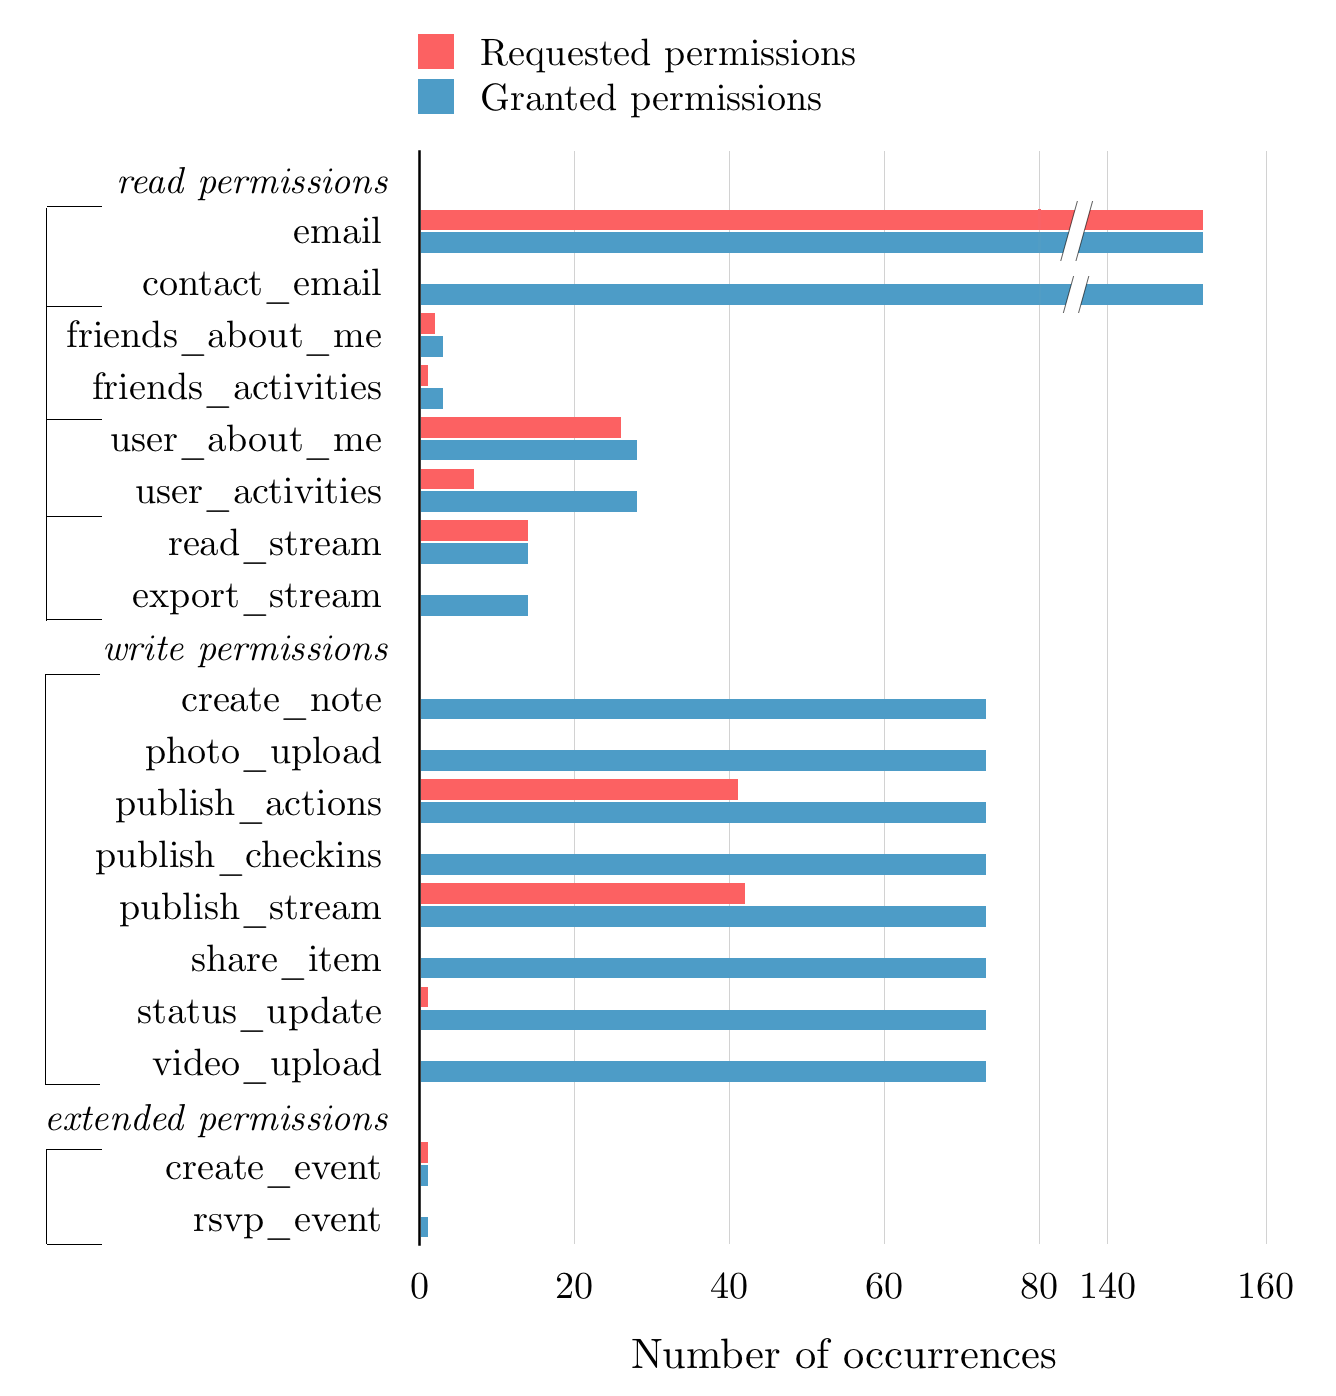
\includegraphics[width=8.5cm]{scope_vs_html_cosn}
  \caption{Permissions requested vs.\ permissions granted for permissions granted in groups, as listed in Table~\ref{table:permgroups}.}
  \label{figure:scopevshtml}
\end{figure}

%The significance of Facebook giving these permissions in groups will be discussed after discussing the way Facebook presents them to the user.
\begin{table*}[htb]
  \centering
  \begin{tabular}{|l|l|l|}
    \hline
    \multicolumn{3}{|l|}{\textbf{Read Permissions:} \textit{Site\_Name will receive the following info\dots}}                                                                                                                                                                                                                                                                                                                                                   \\ \hline \hline
    \textbf{Message}                                                                                                                                                                                                                                                 & \textbf{Permission} & \textbf{Meaning} \cite{fbpermissions}                                                                                                                          \\ \hline
    \multirow{2}{*}{email address}                                                                                                                                                                                                                                   & email               & email                                                                                                                                     \\ \cline{2-3} 
    & contact\_email      & not listed                                                                                                                                \\ \hline
    \multirow{2}{*}{News Feed}                                                                                                                                                                                                                                        & read\_stream        & access my News Feed and Wall                                                                                                              \\ \cline{2-3} 
    & export\_stream       & \begin{tabular}[l]{@{}l@{}}export my posts and make them \\ public. All posts will be exported, \\ including status updates.\end{tabular} \\ \hline
    \multirow{2}{*}{personal description}                                                                                                                                                                                                                            & user\_about\_me     & about me                                                                                                                                  \\ \cline{2-3} 
    & user\_activities    & activities                                                                                                                                \\ \hline \hline
    \multicolumn{3}{|l|}{\textit{...and your friends'\dots}}                                                                                                                                                                                                                                                                                                                                                                               \\ \hline \hline
    \multirow{2}{*}{personal descriptions}                                                                                                                                                                                                                           & friends\_about\_me  & `about me' details                                                                                                                         \\ \cline{2-3} 
    & friends\_activities & activities                                                                                                                                \\ \hline \hline
    \multicolumn{3}{|l|}{\textbf{Write Permissions:} \textit{Site\_Name would like to\dots}}                                                                                                                                                                                                                                                                                                                                                                    \\ \hline \hline
    \textbf{Message}                                                                                                                                                                                                                                                 & \textbf{Permission} & \textbf{Meaning}                                                                                                                          \\ \hline
    \multirow{8}{*}{\begin{tabular}[l]{@{}l@{}}post to Facebook for you.\\ \textit{-- or{\footnotesize *} --}\\ post publicly to Facebook for you.\\ \textit{-- or{\footnotesize *} --}\\ post privately to Facebook for you.\end{tabular}} & create\_note        & create and modify events                                                                                                                  \\ \cline{2-3} 
    & photo\_upload       & add or modify photos                                                                                                                      \\ \cline{2-3} 
    & publish\_actions    & publish my app activity to Facebook                                                                                                       \\ \cline{2-3} 
    & publish\_checkins   & publish checkins on my behalf                                                                                                             \\ \cline{2-3} 
    & publish\_stream     & publish content to my Wall                                                                                                                \\ \cline{2-3} 
    & share\_item         & share items on my behalf                                                                                                                  \\ \cline{2-3} 
    & status\_update      & update my status                                                                                                                          \\ \cline{2-3} 
    & video\_upload       & add or modify videos                                                                                                                      \\ \hline \hline
    \multicolumn{3}{|l|}{\textbf{Extended Permissions:} \textit{Site\_Name would like to\dots}}                                                                                                                                                                                                                                                                                                                                                                 \\ \hline \hline
    \textbf{Message}                                                                                                                                                                                                                                                 & \textbf{Permission} & \textbf{Meaning}                                                                                                                          \\ \hline
    \multirow{2}{*}{manage your events}                                                                                                                                                                                                                              & create\_event       & create and modify events                                                                                                                  \\ \cline{2-3} 
    & rsvp\_event         & RSVP to events                                                                                                                            \\ \hline
  \end{tabular}
  \caption{Message decoder for permissions that are granted in groups. \extendedversion{Decoder tables for all permissions are in Appendix~\ref{appendix:decodetables}.}{} Italic text represents how the permissions are introduced when presented to the user. See Figure~\ref{figure:messageexample} for an example. \\ \footnotesize *Which of the three messages is presented depends on to whom the posts will be visible. This is controlled by the menu in the bottom left of the middle image in Figure~\ref{figure:messageexample}.}
  \label{table:messagegrouped}
\end{table*}
\subsection{How permissions are presented to the user} 
\label{sec:messages} 

As mentioned previously, when the user logs in to a site with Facebook Connect for the first time they are presented with up to three messages from Facebook asking them to approve the read, write, and/or extended permissions.
We reverse-engineered the algorithm for generating the phrase or word in the displayed permissions message that corresponds to each granted permission using our test site and verified that it matched the data observed in our crawl.
Most messages appear reasonably clear.
However, the grouped permissions (see Table~\ref{table:permgroups}) are displayed with just one corresponding word or phrase indicating that \emph{all} the permissions in that group are being requested. Table~\ref{table:messagegrouped} presents these potentially unclear messages and their meaning according to the Facebook Connect documentation \cite{fbpermissions}. \extendedversion{Similar tables for all permissions can be found in Appendix~\ref{appendix:decodetables}.}{}


\subsection{Facebook's response}
\label{sec:fbresponse}

We sent a security bug report to Facebook stating that we could use the \emph{publish\_actions} permission after requesting any other write permission. Facebook Security stated\footnote{Our full correspondence with Facebook is in Appendix~\ref{appendix:correspondence}.} that ``this behavior is by design'' and confirmed that when one permission is requested in the scope, they ``translate them to a broader set of [permissions] which are easier for users to understand'' \cite{fbsecurity}. When asked why this was done for write permissions but not read permissions, they responded that they ``made this change to simplify the experience for developers and for users'' and that ``write permissions are more similar...whereas read permissions are more distinct.'' 
This motivated us to evaluate whether all-or-nothing write permissions are in fact easier for the user to understand.%, which we turn to in the next section.

\extendedversion{}{\vspace{1cm}}
\section{User understanding}
\label{sec:understanding}

The second critical component in effective user control on Facebook Connect is users' comprehension of the messages describing the permissions they're asked to approve.
This is especially important given our findings in Section~\ref{sec:implementation} that all write permissions are grouped together and displayed with a single somewhat-vague message. 
Previous research  by Egelman \cite{egelman} found that 88\% of users have a general understanding of Facebook's read permissions dialogues; however, he studied only the read permissions dialogues.
To our knowledge this is the first study evaluating comprehension of write permissions.
Together with read permissions these make a fascinating natural experiment: are users better able to understand granular (but complicated) read permissions, or simpler (but vaguer) write permissions?
To test this and other aspects of user comprehension, we ultimately conducted three studies:

\begin{enumerate}
  \item One study tested general comprehension of read and write permissions and compared them to each other (see Section~\ref{sec:comparisonsurvey}).\footnote{We decided not to test extended permissions since they are presented similarly to read permissions and are relatively rare (only seven out of the 177 sites requested them).} 
  \item One study tested how site identity affects interpretation of the write permissions message (see Section~\ref{sec:multisite}).
  \item Our final study tested to see if users understand that they are giving access to data regardless of their profile privacy settings (see Section~\ref{sec:privacysurvey}).
\end{enumerate}

\subsection{Methodology}

We conducted our surveys using Amazon Mechanical Turk, a service where workers can be paid to complete simple online tasks. This allowed a large and reasonably diverse response pool for little cost (we paid 10-15 cents per response). (See Section~\ref{sec:limitations} for a discussion of Mechanical Turk's limitations.)
All of our surveys took the basic format of presenting users with real dialogues that they might see when logging in to a site using Facebook Connect and asking questions about what actions that site may take if they authorize the login.


\subsubsection{Pilot studies}

We piloted three different methods of testing user comprehension. After verifying that the respondent had previously seen a Facebook Connect login, all pilots began by presenting the respondent with either a read or write permissions message that they might see when using Facebook Connect. No respondents were presented with both to ensure that no one got the two questions mixed up.
Respondents were then presented with one of the following three question types:

\begin{enumerate}  
  \item A yes/no question asking if the site would be able to do something if they clicked okay, such as view their photos or update their status.
  \item A list of things the site might be able to do if they clicked okay. The user was asked to select all those they thought the site would be able to do.
  \item A free response question asking the user to describe what information they thought the site would be able to do if they clicked okay.
\end{enumerate}

The free response question has the advantage of not prompting the user with any ideas that may not have occurred to them otherwise. However, pilots showed that answers to free response questions were frequently too vague to be useful and that respondents may not have put enough thought into their answers. While this may reflect how users pay little attention to permissions messages in real life when they log in to sites, it is not useful for this survey.
There was no noticeable difference in responses between the yes/no questions and the multiple-selection questions, so we chose the latter to get results about more permissions.

We also experimented with showing the respondent messages from different sites. There was some indication that the site influenced the responses. For example, people appeared more likely to think photo-oriented sites like Flickr would be able to do photo-oriented things, such as uploading photos. To keep our independent variables separate, we conducted two different surveys. The first survey (Section~\ref{sec:comparisonsurvey}) used the site name ``Hooli.com'' (Hooli is a fake tech company in HBO's \emph{Silicon Valley}). The description of the site given to users was a description of a real site, \emph{Splashscore.com}. This was one of the sites piloted and we determined it had an appropriately general-sounding description and could conceivably need a wide variety of permissions. \extendedversion{The way the site was presented to users can be seen in Appendix~\ref{appendix:surveys}.}{} Our second survey (Section~\ref{sec:multisite}) was designed to test write permission comprehension across different sites.

\subsection{Read vs.\ write permissions}
\label{sec:comparisonsurvey}

Our first study tests general comprehension of read and write permissions in such a way that they can be directly compared. For all questions, we used the site name ``Hooli.com'' to eliminate the site name as a variable. Our tests were designed to evaluate the the following null hypotheses:

\begin{hypothesis}\label{hyp:read_equals_random}
Respondents' ability to identify which read permissions they are authorizing is no different than if they were randomly guessing.
\end{hypothesis}
\begin{hypothesis}\label{hyp:write_equals_random}
Respondents' ability to identify which write permissions they are authorizing is no different than if they were randomly guessing.
\end{hypothesis}
\begin{hypothesis}\label{hyp:read_equals_write}
Respondents' ability to identify which read permissions they are authorizing is no different than their ability to identify which write permissions they are authorizing.
\end{hypothesis}
%\begin{enumerate}
 % \item Respondents' ability to identify which read permissions they are authorizing is no different than if they were randomly guessing.
  %\item Respondents' ability to identify which write permissions they are authorizing is no different than if they were randomly guessing.
 % \item Respondents' ability to identify which read permissions they are authorizing is no different than their ability to identify which write permissions they are authorizing.
%\end{enumerate}

This survey was taken by 600 Mechanical Turk workers. All were first asked if they had seen a site use Facebook login before---nearly all had. Half of those who had\footnote{Respondents who had not seen a Facebook Connect login were not given the rest of the survey and were excluded from analysis, but were still paid for their participation.} were presented with Facebook's standard write permissions message followed by 13 options of things they might be giving the site permission to do by clicking okay. Eight of the 13 were taken almost directly from the Facebook Connect documentation's permission descriptions \cite{fbpermissions}, so they were all things the site would be able to do (since Facebook gives all write permissions together). The other five were things the site could not do. They were present not to be tested but to eliminate biases due to an aversion to selecting all available options. The 13 options were presented in 4 different orders\extendedversion{ and can be seen in Appendix~\ref{appendix:writesurveys}.}{.}

The other half were presented with read permissions questions. Since read permissions messages vary, we used messages taken from four different real sites with varying numbers of permissions (\emph{Jabong.com}, \emph{Flickr.com}, \emph{Splashscore.com}, and \emph{TripAdvisor.com}). All were renamed ``Hooli.com.'' Each message was followed with eight or nine options for things the site might be able to do. Four or five options were information on a Facebook profile that the site would be able to see. The other four were either things the site could not see or were write or extended permissions.\footnote{It is difficult to determine what the site cannot see since the user's public profile could contain a lot of information if they have relaxed privacy settings, so only very clear-cut things like seeing private messages could be used.} Again, the incorrect answers were only so the respondent did not have to select all options to be correct. \extendedversion{The four different questions can be seen in Appendix~\ref{appendix:readsurveys}.}{} There are too many different read permissions to effectively test them all without exhausting the respondents with too many questions, so the ones tested are some of the more common ones.

\subsubsection{Read permissions results}

Figure~\ref{figure:readpercents} illustrates the percentage of people who correctly identified that each permission would be given to the requesting site after they clicked okay.\footnote{Only the real permissions being requested are presented. The incorrect answers we made up are not.} Table~\ref{table:readstats} lists the numerical percentages as well as the 2-tailed \emph{p}-value from a binomial test comparing the number of people who correctly identified a permission as being requested to the expected value with random guessing: half of the total number of people who were presented with that permission.

\begin{figure}[tb!]
  \centering
  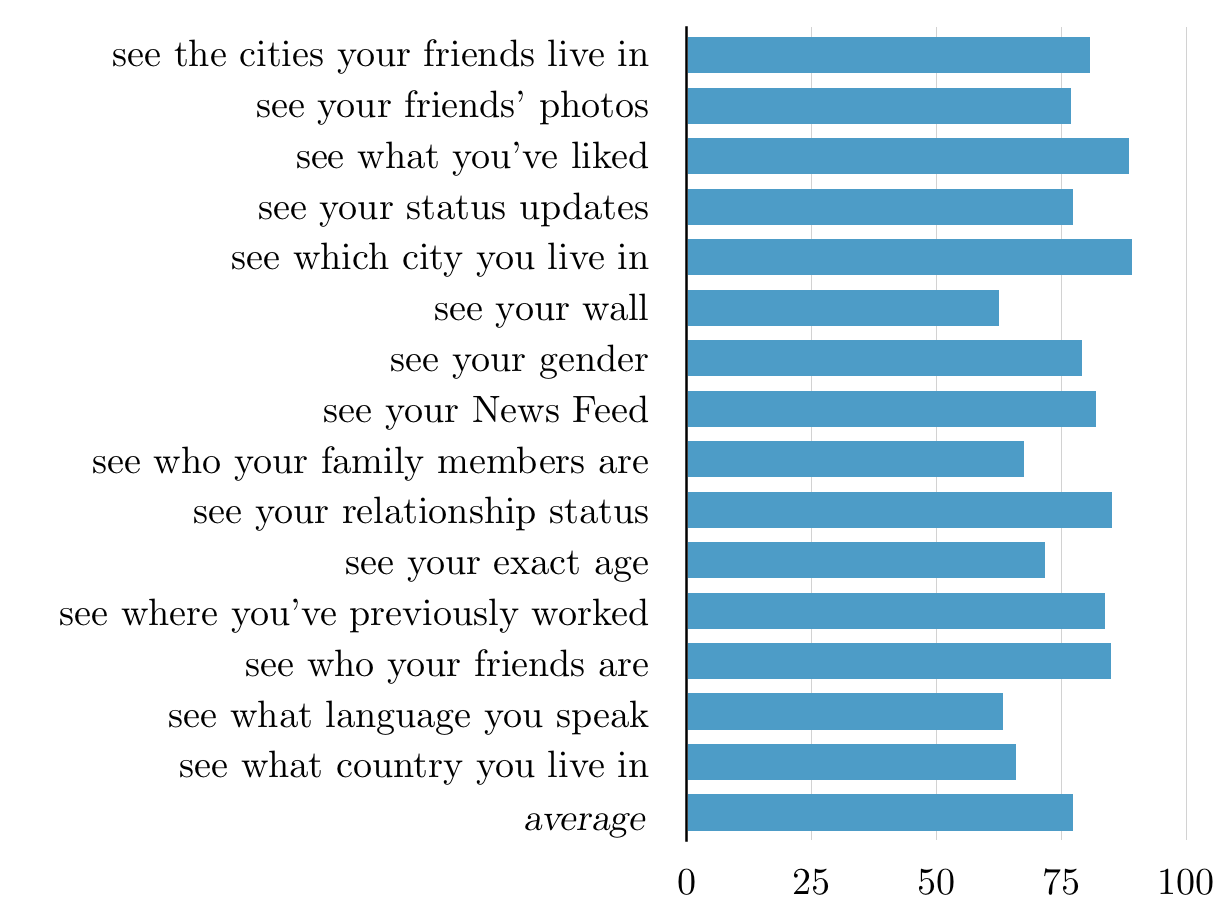
\includegraphics[width=8.5cm]{read_percents_cosn}
  \caption{Percentage of people who correctly identified that each read permission would be granted to the site upon authorization.}
  \label{figure:readpercents}
\end{figure}

\begin{table}[tb!]
  \centering
  \begin{tabular}{|l|l|l|l|}
    \hline
    \textbf{Permission}            & \textbf{N}      & \begin{tabular}[c]{@{}l@{}}\textbf{Percent}\\\textbf{Correct}\end{tabular} & \begin{tabular}[c]{@{}l@{}}\textbf{2-tailed} \\\textbf{\emph{p}-value}\end{tabular}                 \\ \hline \hline
    \begin{tabular}[c]{@{}l@{}}see the cities your \\ friends live in \end{tabular}& 78 & 80.77                                 & 0.000         \\ \hline
    see your friends' photos            & 78 & 76.92                                 & 0.000           \\ \hline
    see what you've liked               & 78 & 88.46                                 & 0.000     \\ \hline
    see your status updates             & 150 & 77.33                                 & 0.000       \\ \hline
    \begin{tabular}[c]{@{}l@{}}see which city you live\\ in\end{tabular}          & 230 & 89.13                                 & 0.000 \\ \hline
    see your wall                       & 72  & 62.50                                             & 0.044               \\ \hline
    see your gender                     & 72 & 79.17                                 & 0.000          \\ \hline
    see your News Feed                  & 72 & 81.94                                 & 0.000         \\ \hline
    \begin{tabular}[c]{@{}l@{}}see who your family \\members are\end{tabular}     & 80 & 67.50                                             & 0.002              \\ \hline
    \begin{tabular}[c]{@{}l@{}}see your relationship\\ status\end{tabular}        & 80 & 85.00                                            & 0.000       \\ \hline
    see your exact age                  & 159 & 71.70                                 & 0.000         \\ \hline
    \begin{tabular}[c]{@{}l@{}}see where you've \\previously worked\end{tabular}  & 80 & 83.75                                            & 0.000       \\ \hline
    see who your friends are            & 79 & 84.81                                 & 0.000       \\ \hline
    \begin{tabular}[c]{@{}l@{}}see what language you\\ speak\end{tabular}         & 79 & 63.29                                 & 0.024               \\ \hline
    \begin{tabular}[c]{@{}l@{}}see what country you\\ live in\end{tabular}        & 79 & 65.82                                 & 0.007              \\ \hline
  \end{tabular}
  \caption{\emph{p}-values for 2-tailed binomial test comparing the number of people who correctly selected each permission to Null Hypothesis~\ref{hyp:read_equals_random} of random guessing.} % should I be putting numbers in this table instead of %?
  \label{table:readstats}
\end{table}

For all tested read permissions, over half of people correctly identified that said permission would be granted based on the message presented. On average, individual permissions were correctly identified 79.72\% of the time. This is comparable to Egelman's \cite{egelman} conclusion that 88\% of users understand generally which permissions are being requested.

Null Hypothesis~\ref{hyp:read_equals_random}, that respondents' ability to identify which read permissions they are authorizing is no different than if they were randomly guessing, can be rejected for all but two permissions with $p < .01$,  suggesting that users have a significantly better understanding of which read permissions they are granting than if they were randomly guessing.
We can also reject the possibility that users simply marked every survey option as visible to the website: an average of 81.96\% of users correctly identified each of the options that would not be visible to the site. Null Hypothesis~\ref{hyp:read_equals_random} for each of these options can be rejected with $p < .01$.

Null Hypothesis~\ref{hyp:read_equals_random} for ``see what language you speak'' can be rejected with $p < .03$ and for ``see your wall'' with $p < .05$. A $G$-test\footnote{The $G$-test is a likelihood-ratio statistical test of independence applicable in the same cases as a $\chi^2$-test, but with lower approximation error in nearly all cases than the more traditional Pearson's $\chi^2$-test.} shows that respondents were worse at identifying ``see your wall'' than ``see your status updates'' (which had an accuracy rate roughly equal to the average) with $p < .04$ and a $G$-test statistic of 4.528. Recall that seeing one's Wall and seeing one's News Feed are both granted by the \emph{read\_stream} permission but the message presented to the user says only ``News Feed'' (see Section~\ref{sec:investigationdiscussion}). This may have been the cause of some confusion. Respondents were also worse at identifying ``see what language you speak'' with $p < .04$ and a $G$-test statistic of 4.338, but the reason for this is unclear.

\subsubsection{Write permissions results}

Figure~\ref{figure:writepercents} illustrates the percentage of people who correctly identified that each permission would be given to the requesting site after they clicked okay. Table~\ref{table:writestats} lists the numerical percentages as well as the 2-tailed \emph{p}-value from a binomial test comparing the number of people who correctly identified a permission as being requested to Null Hypothesis~\ref{hyp:write_equals_random}, that user's understanding would be equivalent to random guessing.

\begin{figure}[tb!]
  \centering
  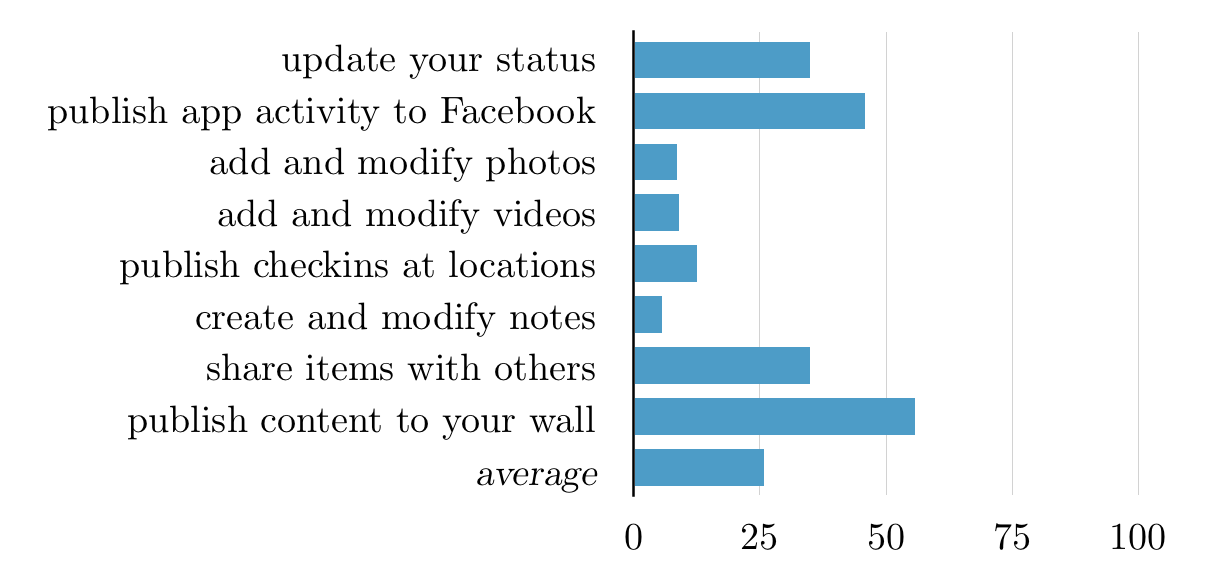
\includegraphics[width=8.5cm]{write_percents_cosn}
  \caption{Percentage of people who correctly identified that each permission would be given to the site upon authorization.}
  \label{figure:writepercents}
\end{figure}

\begin{table}[tb!]
  \centering
  \begin{tabular}{|l|l|l|}
    \hline
    \textbf{Permission}              & \begin{tabular}[c]{@{}l@{}}\textbf{Percent}\\\textbf{Correct}\end{tabular} & \begin{tabular}[c]{@{}l@{}}\textbf{2-tailed}\\ \textbf{\emph{p}-value}\end{tabular}  \\ \hline \hline
    update your status               & 34.88         & 0.000                                                         \\ \hline
    \begin{tabular}[c]{@{}l@{}}publish app activity to \\ Facebook\end{tabular} & 45.85         & 0.166                                                                \\ \hline
    add and modify photos            & 8.64         & 0.000           \\ \hline
    add and modify videos            & 8.97         & 0.000            \\ \hline
    publish checkins at locations    & 12.62          & 0.000                      \\ \hline
    create and modify notes          & 5.65         & 0.000 \\ \hline
    share items with others          & 34.88         & 0.000       \\ \hline
    publish content to your wall     & 55.81         & 0.050      \\ \hline
  \end{tabular}
  \caption{\emph{p}-values for 2-tailed binomial test comparing the number of people who correctly selected each permission to Null Hypothesis~\ref{hyp:write_equals_random} of random guessing. $N$ = 301 for all permissions.} 
  \label{table:writestats}
\end{table}

For all permissions except for ``publish content to your wall,'' fewer than half of respondents answered correctly. For all of those except ``publish app activity to Facebook,'' Null Hypothesis~\ref{hyp:write_equals_random}, that respondents' ability to identify which write permissions they are authorizing is no different than if they were randomly guessing, can be rejected with $p < .01$. That is, for these six permissions, people would have been significantly more likely to correctly identify whether they were granting the permission by randomly guessing.

The \emph{p}-value for ``publish app activity to Facebook'' is too high to reject Null Hypothesis~\ref{hyp:write_equals_random} with a reasonable level of confidence. 

Over half of people correctly identified that the site would be able to ``publish content to [their] wall,'' and Null Hypothesis~\ref{hyp:write_equals_random} can be rejected with $p < .05$. People may have a better idea that this permission is being granted than if they were randomly guessing. 

Worth noting is that the two permissions people did best with (``publish content to your wall'' and ``publish app activity to Facebook'') are also the vaguest. (These are the \emph{publish\_stream} and \emph{publish\_actions} permissions that are intended to give nearly all publishing permissions.) Because they are so vague, the fact the more people selected them correctly probably does not mean that they fully understand the specific things the site can post on their profile---they include the functions of the other permissions, which most users were not successful at identifying.

\subsubsection{Comparison of read and write permissions}

It appears evident at this point that users understand read permissions messages significantly better than they understand write permissions messages: Respondents correctly identified whether a read permission would be granted 79.72\% of the time, whereas write permissions were only correctly identified 25.91\% of the time.

To evaluate Null Hypothesis~\ref{hyp:read_equals_write}, that respondents' ability to identify which read permissions they are authorizing is no different than their ability to identify which write permissions they are authorizing, we assigned a ranking to each respondent based on the percentage of permissions they correctly identified\footnote{This counts only the real permissions and not the incorrect options since those were artificially created.} and separated them into two groups, one for those asked about read permissions and one for those asked about write permissions.  A Mann-Whitney $U$ test of these two groups allows us to reject Null Hypothesis~\ref{hyp:read_equals_write} with $p < 0.001$ and a test statistic of $U=9163$.

\subsection{Influence of relying site}
\label{sec:multisite}

As previously mentioned, our pilot surveys indicated that the site identity may influence how people interpret the write permissions message. We performed a separate survey with 300 Mechanical Turk workers to test this. The format of the survey was identical to the write permissions questions in the first survey and we provided the same options for the user to select. However, instead of using ``Hooli.com'' as the website in question, one third of respondents were presented with \emph{Flickr.com} (a photo and video sharing site), one third with \emph{TripAdvisor.com} (a travel site), and one third with \emph{iFlikeU.com} (an anonymous messaging site). (Since there is only one write permissions message, the message presented to the user in all cases was identical aside from the site name and description.)

The results of this survey can be statistically analyzed with a $G$-test to see if the number of respondents who thought each permission would be granted varied across the four sites (the three mentioned here plus the data from ``Hooli.com'' from the first survey). Our null hypothesis is: 

\begin{hypothesis}\label{hyp:site_identity}
The relying site's identity does not affect how respondents interpret a requested permission.
\end{hypothesis}

\subsubsection{Results}

Figure~\ref{figure:multipercents} illustrates the percentage of people who correctly identified that each permission would be given to each site after they clicked okay. Table~\ref{table:multistats} lists the numerical percentages as well as the \emph{p}-values from a $G$-test comparing the variation in number of correct selections for each permission across all four sites.

\begin{figure}[tb!]
  \centering
  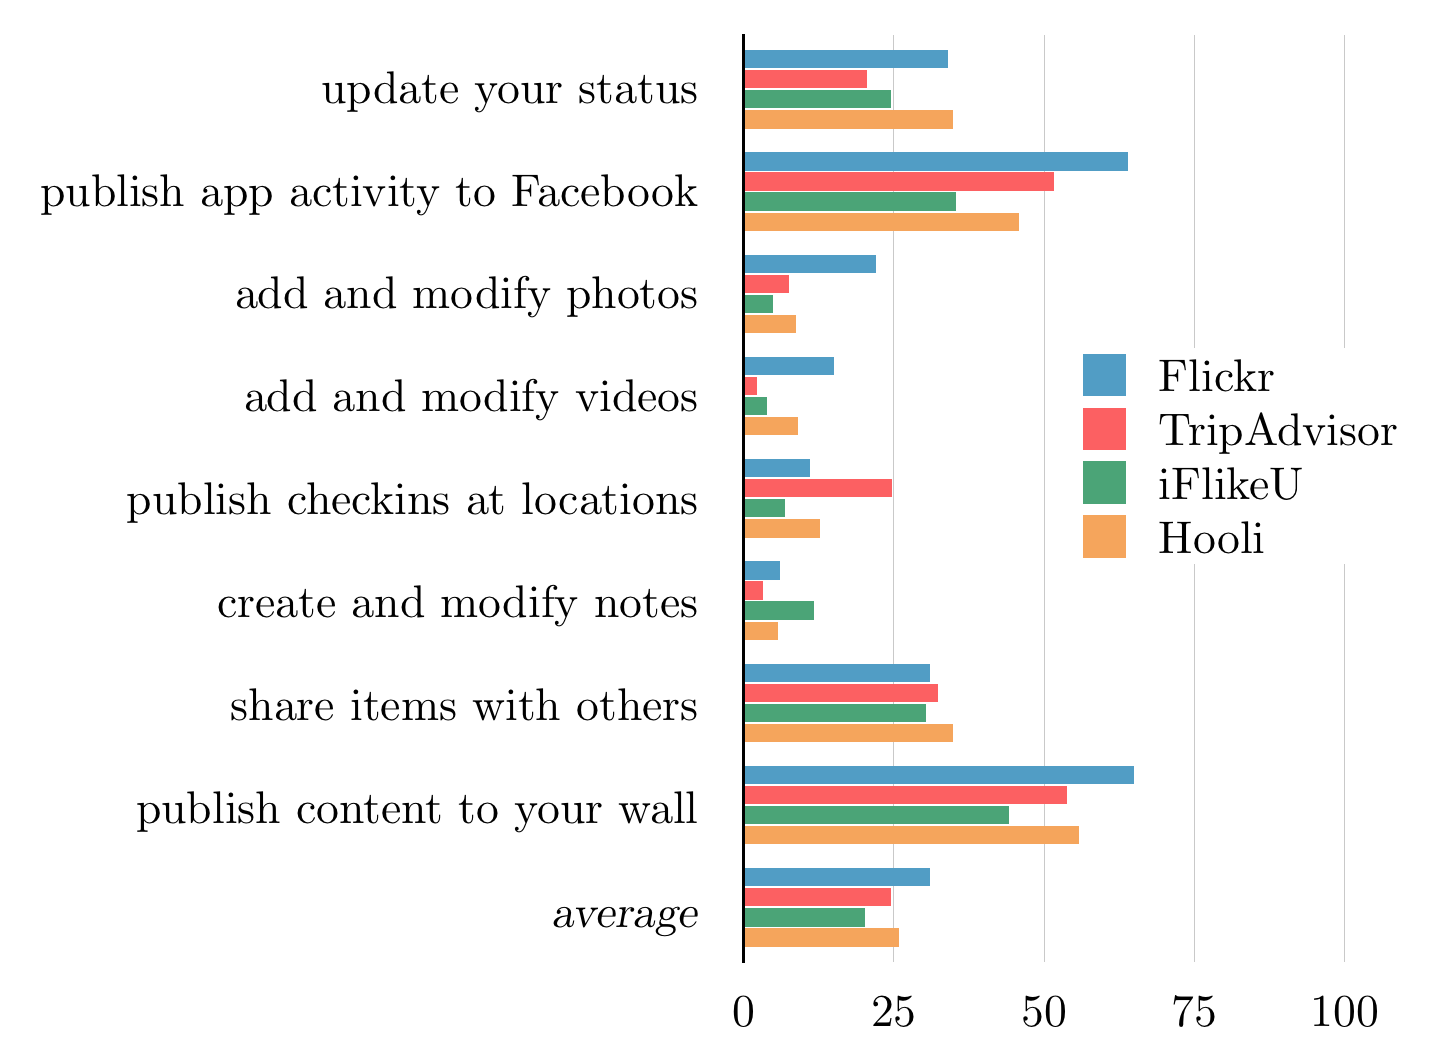
\includegraphics[width=8.5cm]{multi_percents_cosn}
  \caption{Percentage of people who correctly identified that each permission would be given to the site upon authorization for four sites.}
  \label{figure:multipercents}
\end{figure}

\begin{table*}[htpb]
  \centering
  \begin{tabular}{|l|l|l|l|l|l|l|}
    \hline
    \multirow{2}{*}{\textbf{Permission}} & \multicolumn{4}{l|}{\textbf{Percent Correct}}                                                                                                                                                                                                             & \multirow{2}{*}{\textbf{\begin{tabular}[c]{@{}l@{}}$G$-test\\ statistic\end{tabular}}} & \multirow{2}{*}{\textbf{p-value}} \\ \cline{2-5}
    & \begin{tabular}[c]{@{}l@{}}Flickr \\ ($N$ = 100)\end{tabular} & \begin{tabular}[c]{@{}l@{}}TripAdvisor \\ ($N$ = 93)\end{tabular} & \begin{tabular}[c]{@{}l@{}}iFlikeU \\ ($N$ = 102)\end{tabular} & \begin{tabular}[c]{@{}l@{}}Hooli \\ ($N$ = 301)\end{tabular} &                                                                                      &                                   \\ \hline\hline
    update your status                   & 34                                                          & 20.43                                                           & 24.51                                                        & 34.88                                                      & 8.662                                                                                & 0.034                             \\ \hline
    publish app activity to Facebook     & 64                                                          & 51.61                                                           & 35.29                                                        & 45.85                                                      & 16.733                                                                               & 0.001                             \\ \hline
    add and modify photos                & 22                                                          & 7.53                                                            & 4.90                                                         & 8.64                                                       & 15.185                                                                               & 0.002                             \\ \hline
    add and modify videos                & 15                                                          & 2.15                                                            & 3.92                                                         & 8.97                                                       & 11.783                                                                               & 0.008                             \\ \hline
    publish checkins at locations        & 11                                                          & 24.73                                                           & 6.86                                                         & 12.62                                                      & 10.937                                                                               & 0.006                             \\ \hline
    create and modify notes              & 6                                                           & 3.23                                                            & 11.76                                                        & 5.65                                                       & 4.783                                                                                & 0.188                             \\ \hline
    share items with others              & 31                                                          & 32.26                                                           & 30.39                                                        & 34.88                                                      & 0.706                                                                                & 0.872                             \\ \hline
    publish content to your wall         & 65                                                          & 53.76                                                           & 44.12                                                        & 55.81                                                      &    8.208                                                                                  & 0.042                             \\ \hline
  \end{tabular}
  \caption{\emph{p}-values for $G$-test comparing the number of people who correctly selected each permission across four sites to Null Hypothesis~\ref{hyp:site_identity} of no difference between sites.}
  \label{table:multistats}
\end{table*}

For ``publish app activity to Facebook,'' ``add and modify photos,'' ``add and modify videos,'' and ``publish checkins at locations,'' Null Hypothesis~\ref{hyp:site_identity}, that the relying site's identity does not affect how respondents interpret a requested permission, can be rejected with $p < .01$. More respondents thought Flickr would be able to add and modify photos and videos compared to other sites, which is reasonable since it is a photo and video sharing site. Likewise, many more people thought that TripAdvisor would be able to publish checkins at locations---a logical thing for a travel site to do.

Null Hypothesis~\ref{hyp:site_identity} can be rejected for ``update your status'' with $p < .04$ and ``publish content to your wall'' with $p < .05$. It cannot be rejected for ``share items with others'' nor ``create and modify notes'' with a reasonable level of confidence.

%\textbf{TODO: Should this be moved to discussion?} It appears that users' perception of the write permissions message is influenced by the site identity for some permissions. This further highlights the vagueness of the message---although it means the same thing for every site, users think it means something different on different sites.


\subsection{Influence of privacy settings}
\label{sec:privacysurvey}

In one pilot survey of the free response format, a respondent stated that the site would gain access to only a limited number of permissions because their Facebook settings prevented them from accessing the rest. This suggests a lack of understanding of how the read permissions work: A site can access nearly everything that is public with only the \emph{public\_profile} permission \cite{fbprivacyfaq}. By granting the site additional permissions, a user is giving the site permission to access that information regardless of the user's privacy settings. Using the test site, we confirmed that we could see all user photo albums regardless of their privacy settings with the \emph{user\_photos} permission.

We surveyed 100 additional Mechanical Turk respondents to see if this confusion was widespread. The survey presented the user with the permission message for \emph{Imgur.com}, which requests the \emph{user\_photos} permission. Users were asked to identify which photo albums Imgur would be able to see if they clicked okay. The options were those marked as visible to the public, those marked as visible to friends, and those marked as visible to only them (the correct answer is all three). \extendedversion{The survey can be seen in Appendix~\ref{appendix:readsurvey2}.}{}

Our null hypothesis in this experiment is:

\begin{hypothesis}\label{hyp:privacy_setting}
Respondents are equally likely to indicate that data can be read regardless of its privacy setting.
\end{hypothesis}

\subsubsection{Results}

%The results of our survey comparing read and write permissions (Section~\ref{sec:comparisonsurvey}) indicated that read permissions are understood decently well. However, the additional survey testing whether people understand that they are giving permission to view things that are not marked as ``public'' (see Section~\ref{sec:privacysurvey}) suggests that they do not understand this aspect.

Figure~\ref{figure:privacypercents} illustrates the percentage of people who correctly identified that Imgur.com would be able to see their photo albums with various privacy settings if they clicked okay.
%Table~\ref{table:privacystats} lists the numerical percentages as well as the 2-tailed \emph{p}-value from a binomial test comparing the number of people who correctly identified that a privacy level was visible compared to Null Hypothesis~\ref{hyp:privacy_setting} of random guessing: half of the total number of people who were given the survey.
It appears people are generally aware that they are giving access to their photo albums that are marked as public. However, they are generally unaware that they are also giving access to their photo albums that are marked as visible to their friends or only to themselves. 

\begin{figure}[tb!]
  \centering
  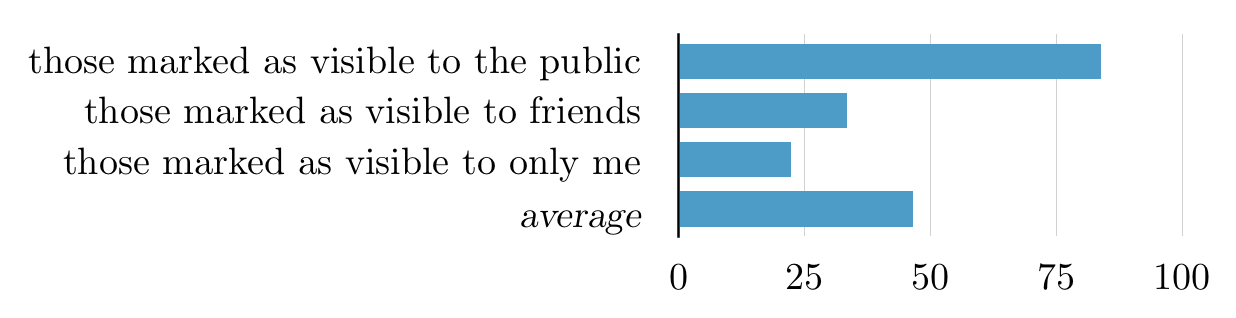
\includegraphics[width=8.5cm]{privacy_percents_cosn}
  \caption{Percentage of people who correctly identified that Imgur.com would be able to see their photo albums of each privacy level upon authorization.}
  \label{figure:privacypercents}
\end{figure}

\begin{comment}
\begin{table}[tb!]
  \centering
  \begin{tabular}{|l|l|l|}
    \hline
    \textbf{Privacy Setting}              & \begin{tabular}[c]{@{}l@{}}\textbf{Percent}\\\textbf{Correct}\end{tabular} & \begin{tabular}[c]{@{}l@{}}\textbf{2-tailed}\\ \textbf{\emph{p}-value}\end{tabular}     \\ \hline \hline
    \begin{tabular}[c]{@{}l@{}}those marked as visible \\to the public \end{tabular} & 83.84         & 0.000 \\ \hline
    \begin{tabular}[c]{@{}l@{}}those marked as visible \\to friends\end{tabular}    & 33.33         & 0.001           \\ \hline
    \begin{tabular}[c]{@{}l@{}}those marked as visible \\to only me\end{tabular}    & 22.22         & 0.000      \\ \hline
  \end{tabular}
  \caption{\emph{p}-values for 2-tailed binomial test comparing the number of people who correctly selected each privacy level to Null Hypothesis~\ref{hyp:privacy_setting} FIXME. $N$ = 99.} 
  \label{table:privacystats}
\end{table}

\begin{table}[tb!]
  \centering
  \begin{tabular}{|l|l}
    \hline
    \textbf{Privacy Setting}              & \textbf{Percent Correct} \\ \hline \hline
    those marked as visible to the public & 83.84   \\ \hline
    \begin{tabular}[c]{@{}l@{}}those marked as visible \\to friends\end{tabular}    & 33.33            \\ \hline
    \begin{tabular}[c]{@{}l@{}}those marked as visible \\to only me\end{tabular}    & 22.22      \\ \hline
  \end{tabular}
  \caption{\emph{p}-values for 2-tailed binomial test comparing the number of people who correctly selected each privacy level to Null Hypothesis~\ref{hyp:privacy_setting} FIXME. $N$ = 99.} 
  \label{table:privacystats}
\end{table}
\end{comment}

Using a $G$-test with three degrees of freedom to compare all three test conditions, Null Hypothesis~\ref{hyp:privacy_setting}, that respondents are equally likely to indicate that data can be read regardless of its privacy setting, can be rejected with $p < .001$ based on a $G$-test statistic of 86.31.
Comparing each pair of conditions in turn using a $G$-test with two degrees of freedom, we can conclude with $p < .001$ that participants were significantly more likely to believe photos marked ``visible to the public'' could be read than either photos marked ``visible to friends'' or ``visible to only me''.
However, we cannot conclude with high confidence ($p \approx .12$) that participants were significantly more likely to believe photos marked ``visible to friends'' could be read than photos marked ``visible to only me''.
Thus we can reject Null Hypothesis~\ref{hyp:privacy_setting} in general and conclude that users do believe privacy settings impact visibility of data to third-party sites, we cannot conclude if the specific privacy settings (visible to friends or only to the user) had a significant impact on user understanding.

Although our first set of surveys and Egelman's study \cite{egelman} indicated that read permissions are understood decently well, this study suggests that these results may not actually be entirely representative of user understanding: although people know which types of information they are granting access to, most do not realize they are giving access to that information even if they have marked it with a privacy level other than public.
%However, this section of our study was performed on a relatively small scale (one website with one permission and 100 responses). A future study could test this comprehensively.


\subsection{Limitations}
\label{sec:limitations}

There are several possible limitations to our surveys:

\begin{itemize}
  \item As discussed previously, by giving respondents several options to select we suggested possible things the site could do that may not have occurred to them otherwise. In addition, in order to respond to our questions they may have paid more attention to the permissions dialogues than they normally would have. As a result, our survey may indicate that users are more aware of what permissions are being requested than they are in practice.
  \item If read and write permissions are fundamentally different in some non-obvious way, it may be invalid to compare understanding of read permissions to understanding of write permissions. It is possible that users would understand write permissions even more poorly if they were presented granularly rather than all-or-nothing.
  \item There may be some demographic bias in using Mechanical Turk to collect responses. We did not collect demographic information from respondents although we did restrict respondents to the United States (this was the only restriction we placed on respondents). Our use of Mechanical Turk is justified by previous research finding that ``[Mechanical Turk] participants produced reliable results that are consistent with previous decision-making research'' \cite{mturkreliability}. The most relevant concern they raise is of respondents not paying enough attention and becoming fatigued in longer surveys; the short length of our surveys hopefully ameliorated that to some degree. In addition, users are known to pay little attention to permissions messages in practice~\cite{egelman}.
  \item When asking users which permissions were being granted, we had to make up some fake options so users did not have to select every option to be correct. If we did a poor job, this could have influenced results by distracting or unsettling users. We did not count these made up permissions in our statistical analysis for this reason.
\end{itemize}


%\subsection{Analysis of survey results}

%Our survey showed that users are significantly better than random guessing at identifying which read permissions are being requested. However, they are significantly worse at identifying write permissions. The additional survey demonstrated that users may not understand that they are allowing data to be viewed regardless of its privacy settings.

\section{Discussion}

% BEGIN WITH THIS IF WE JUST FOCUS ON COMPARISON: Our studies indicate that users' understanding of write permissions messages is significantly worse than their understanding of read permissions messages.

Our study indicates that users have a decent understanding of read permissions messages but a significantly worse understanding of write permissions messages. As discussed in Section~\ref{sec:fbresponse}, Facebook claims that all-or-nothing write permissions are easier for the user to understand. However, comparison with the very granular read permissions suggests that users understand specific, distinct permissions better.

We also observe that grouped permissions cause confusion for developers who may receive more permissions than intended due to grouping of permissions.
This appears contrary to Facebook's stated advice to developers that they should ``only ask for the permissions that are essential to an app [or site]'' \cite{fbpermsinstructions}. Facebook's own research has demonstrated that ``the more permissions an app requests, the less likely it is that people will use Facebook to log into [that] app''\cite{fbpermsinstructions}.
But because Facebook Connect often grants more permissions than the developer requested (even just by always granting \emph{public\_profile} and \emph{user\_friends}), the developer may have no choice but to receive unnecessary permissions.

We consider several possible explanations for why the system may be architected this way.

\subsection{Evolution over time}

Some of our findings around the permissions API appear likely to be artifacts of the API's evolution, many of which appear harmless.
For example, two permissions for reading an email address exist (\emph{email} and \emph{contact\_email}) and grouping them seems sensible.

%\subsection{Why does Facebook handle permissions this way?}
\label{sec:investigationdiscussion}

\begin{comment}
This section has explored the way a set of permissions is transformed from the time when the developer designs the site to request permissions to the point where the permissions are presented to the user for approval. The developer requests a certain set of permissions and then the Facebook Connect API may add additional permissions to that set because certain permissions are always granted in groups. These are the permissions that will be given to the site should the user approve them. When the user is asked for approval, they are presented with a message that can be broken down into pieces representing each permission or group of permissions.

But does it actually make a difference that some permissions are grouped together in this way? Combining \emph{create\_event} and \emph{read\_event} and presenting them as ``manage your events'' seems reasonable, as does combining \emph{email} and \emph{contact\_email}, since it is unclear what the difference would be. Although the explanation of \emph{export\_stream} is not very clear, it appears reasonable to combine it with \emph{read\_stream}. The only obvious issue is that the documentation states that \emph{read\_stream} allows access to the News Feed and Wall \cite{fbpermissions}, whereas the message presented to the user says only ``News Feed.''

Combining \emph{user\_about\_me} and \emph{user\_activities} and calling it ``personal description'' (as well as the similar combination of \emph{friends\_about\_me} and \emph{friends\_activities}), however, may be confusing. These two do not intuitively go together, and calling them ``personal description'' hides the presence of \emph{user\_activities}. Potentially the most confusing is the combination of all eight write permissions into one group that is presented as ``post to Facebook for you.'' Users are likely unaware of the many different things they are allowing the site to do to their profile by clicking okay. 
\end{comment}

%Ideally, the system would not be so convoluted. Only the permissions requested by the developer would ever be granted to the site, and all of these permissions would be presented to the user individually. This could make it much easier for users to understand what permissions they are granting a site when they log in. 
%Our studies determined that all-or-nothing write permissions are actually more confusing for users. So why does Facebook group them?

 %Even forcing every site to request the \emph{public\_profile} and \emph{user\_friends} permissions is too much: For many login implementations, the site may need nothing more than a way to identify the user, such as by an email address or an id number. In such cases, the default permissions are unnecessary and may deter people from using the Facebook Connect system.

It appears that the reason that all write permissions are presented together is that Facebook is gradually eliminating the distinction between different types of publishing under the hood. The description in the documentation for \emph{publish\_actions} is ``publish my app activity to Facebook'' and the description for \emph{publish\_stream} is ``publish content to my Wall'' \cite{fbpermissions}. These are quite vague, and seem as though they could encompass nearly anything. A blog post from a Facebook employee \cite{publishperms} helps explain these permissions: They are essentially the same thing (and are being merged into one) and allow a site to do any type of publishing to Facebook. The post mentions that they can be used to upload a photo, which one may have suspected required the \emph{photo\_upload} permission. Another post from a Facebook employee mentions that developers should only request \emph{publish\_actions} because it encompasses all other write permissions in an effort to ``simplify the model'' \cite{clarity}. Furthermore, Facebook's Graph API lists \emph{publish\_actions} as the permission needed for all API calls that involve publishing \cite{fbapi}.

This transition towards only one type of publishing is visible to anyone who has used Facebook for several years: updating one's status and uploading a photo used to be distinct actions, but now they are both performed by creating a post on one's Timeline. Perhaps at one point the six granular write permissions (\emph{create\_note}, \emph{upload\_photos}, \emph{upload\_videos}, \emph{publish\_checkins}, \emph{share\_item}, \emph{status\_update}) were the only write permissions. The read and extended permissions that are presented in groups may stem from similar changes in Facebook's structure and it may no longer be possible to separate them. %However, these changes may make the Facebook Connect authentication process less clear to users. Section~\ref{sec:understanding} will explore whether they do.

It is understandable that changes in the structure of Facebook necessitate changes in the Facebook Connect API to keep it simple and consistent. However, our results suggest user control may significantly harmed for the sake of simplicity. This threat does not appear purely academic, as there are many malicious Facebook apps that abuse the permissions they are given \cite{isappsafe,frappe}.

\subsection{Privacy salience}

It is also possible that Facebook has evolved towards having a vague write permissions message as a strategy to decrease \textit{privacy salience}~\cite{BP09}. If users thought too many permissions were being granted, they may not use the app or the Facebook Connect platform in general. A vague message allows developers to receive more permissions without losing users.

Evidence that this may be Facebook's intention can be seen by comparing the current write permissions messages to those from the previous implementation of Facebook Connect. As mentioned previously, 26 of the 203 websites we crawled used an older implementation. Table~\ref{table:oldmessages} presents a sampling of the messages we saw. These messages may be misleading since they provide examples of what the site can post based on the specific site even though all sites in the table request only \emph{publish\_actions}. However, these messages do distinctly identify several things the sites can post, unlike the vague messages in the current implementation. Facebook's choice to eliminate these descriptions may indicate an attempt to be less clear about what permissions are actually being granted.

By itself, limiting privacy salience cannot be a complete explanation because read permissions remain relatively detailed.
It may be that read permissions are less concerning to users as write permissions can affect the user's profile on Facebook itself, so Facebook is less motivated to obscure them.
Alternatively, it may be the case that read permissions are in fact more sensitive, since data cannot be un-read whereas unwanted posts from a third-party can be deleted.
In this case, it may be that Facebook has decided that its more important to clearly indicate read permissions up front, whereas it isn't worth concerning users with detailed write permissions since posts can be deleted later.
% However, it's possible users are less sensitive to granting read permissions whereas detailed write permissions are more concerning, meaning there is more obscure to downplay the latter. 

\begin{table}[h!]
  \centering
  \begin{tabular}{|l|l|}
    \hline
    \textbf{Site}      & \begin{tabular}[c]{@{}l@{}}\textbf{Write Permissions} \\ \textbf{Message}\end{tabular}                                                                                                              \\ \hline \hline
    Starpires.com      & \begin{tabular}[c]{@{}l@{}}This app may post on your\\ behalf, including status\\ updates, photos and more.\end{tabular}                         \\ \hline
    PioneerLegends.com & \begin{tabular}[c]{@{}l@{}}This app may post on your\\ behalf, including collections\\ you completed, miles you \\collected and more.\end{tabular} \\ \hline
    Stratego.com       & \begin{tabular}[c]{@{}l@{}}This app may post on your\\ behalf, including achievements\\ you earned and more.\end{tabular}                        \\ \hline
    OpenShuffle.com    & \begin{tabular}[c]{@{}l@{}}This app may post on your\\ behalf, including your high\\ scores and more.\end{tabular}                               \\ \hline
    Fupa.com           & \begin{tabular}[c]{@{}l@{}}This app may post on your\\ behalf, including games you\\ played and more.\end{tabular}                               \\ \hline
  \end{tabular}
  \caption{Write permissions messages from sites using an older version of Facebook Connect. All sites are gaming sites. The only write permission requested is \emph{publish\_actions}.} 
  \label{table:oldmessages}
\end{table}

\subsection{Ineffectiveness of user choice}

It is possible that write messages are vague because users are unable to completely understand them (or simply do not pay attention to them~\cite{egelman}), so Facebook has decided it is better off protecting user privacy by policing developers.

Facebook has publicly attempted to address how general write permissions are by placing responsibility on the developer. The aforementioned Facebook blog post explaining the \emph{publish\_stream} and \emph{publish\_actions} permissions~\cite{publishperms} states that since anything can be shared, ``it will continue to be the developer's responsibility to make it clear to the user what content will be shared back to Facebook.'' Facebook's policy was updated to read: ``If a user grants [the developer] a publishing permission, actions [the developer takes] on the user's behalf must be expected by the user and consistent with the user's actions within [the] app.'' This is especially important since our survey showed that users' interpretation of the write permissions message is influenced by the identity of the site even though there is no difference in the permissions being granted. As of the time of this writing, however, this is no longer mentioned in the Facebook policy~\cite{fbpolicy}. 


%\section{Comparison to other SSO implementations}

%We wanted to compare the way Facebook Connect presents permissions with other SSO implementations. However, the Twitter \cite{twitterdocs} and Google \cite{googledocs} implementations are not directly comparable. Neither offers near as many permissions as Facebook Connect does. Google has no write permissions at all and Twitter does not separate the read and write permissions so a user has to approve both to log in. In addition, both perform the OAuth authorization on the backend so the permissions being requested are not visible in the HTML as they are with Facebook Connect's JavaScript SDK.

%Perhaps the most comparable SSO implementations are older versions of Facebook Connect. However, like Twitter, Facebook Connect previously did not separate the read and write permissions. This was changed in 2013 due to complaints of too many apps posting on user's profiles \cite{writeseparate}. 

%The write permissions messages in the older implementations were formatted differently. As mentioned previously, 26 of the 203 websites we crawled used an older implementation. Table~\ref{table:oldmessages} presents a sampling of the messages we saw. These messages appear to do a better job indicating what the site can actually post since they provide examples. However, they may be misleading since they provide examples based on the specific site even though all sites in the table request only \emph{publish\_actions}. Even though the site may be most likely to post what the message suggests, it can still post anything else.

\section{Future areas for research}

This research could be extended in a number of directions.

\begin{itemize}
  \item The results of our survey testing whether users understand that sites are getting access to their information even if it is marked as private (see Figure~\ref{figure:privacypercents}) indicate that there is room for more research in the area. This should be tested with a variety of different permissions. One could also experiment with ways to make it clear to the user that all of their information is being shared, regardless of the privacy settings.
  \item We previously mentioned that our survey included options of things the sites could not actually do so the respondent would not have to select all options to be correct. However, many people selected these fake options. One could research what permissions users think are being requested beyond what is actually being requested. This is an important area of research because people may be unwilling to use the SSO service if they think too many permissions are being given.
  \item It is clear that users do not understand the full range of write permissions being requested. However, Egelman \cite{egelman} determined that users make their decision to use Facebook Connect or not before they see the permissions requested. Egelman only tested read permissions, though. A similar study could see how the presence of write permissions affects users' decisions to use Facebook Connect. 
  \item We observed that users understand the granular read permissions better than the single write permission. One could test whether granular write permissions are in fact more clear to users than the current system. 
%We did not test this because the success of the study would depend on the researcher's ability to make up plausible granular write permissions.
%  which write permissions are being requested and varying the number of write permissions requested affects whether users are willing to use the system.
\end{itemize}

\section{Related work}
\label{sec:research}

Many researchers have studied the security and permissions systems of various apps\footnote{The Facebook Connect SSO system uses the same system as native Facebook apps---creating a Facebook login on a website requires creating a Facebook app \cite{fbexample}.} and SSO systems. Sun and Beznosov \cite{devildetails} uncovered vulnerabilities in many major OAuth SSO implementations. Chaabane et al. \cite{chaabane} and Huber et al. \cite{appinspect} identified information leaks in Facebook and RenRen apps. There have also been several studies of what permissions sites request, such as Frank et al.'s study in which Facebook apps were grouped into categories based on the permissions they request \cite{miningpermissions}.

Some studies have tested user comprehension of SSO systems as well. A 2011 audit of Facebook Ireland looked at, among other things, how clearly the Facebook app system is presented to users. It also states that it ``is not possible for an application to access personal data over and above that to which an individual gives their consent or enabled by the relevant settings''---that is, Facebook's permissions do appropriately limit what data an app can access \cite{irishaudit}.

Sun et al. studied user understanding of the authentication process in general---for example, whether users understood that the site they are logging in to cannot see the password for the identity provider (Facebook, Google, etc.) \cite{ssoperspective}. The study most directly related to ours is Egelman \cite{egelman}, which studied whether users were willing to use Facebook Connect and how well they understand (and how much they pay attention to) the permissions messages. Egelman concluded that 88\% of users have a general understanding that their profile information will be shared with the site they are logging in to, but that they typically do not pay attention to the specifics of the dialogues and do not make their decision whether to use Facebook Connect based on which permissions are being requested.

Our study differs from previous studies by determining what specific permissions correspond to the messages presented to the user and by evaluating user comprehension of these permissions. This lets us answer most precisely whether users understand exactly what information they are sharing by using Facebook Connect. In addition, Egelman only looked at read permissions. We found that write permissions are much more confusing to users.


\section{Concluding Remarks}

To maximize security and to ensure users feel comfortable using Facebook Connect, developers should minimize the number of permissions they request and the permissions should be presented to the user as clearly as possible. On both fronts, Facebook Connect could be improved.

When a developer designs their site to request certain permissions through Facebook Connect, the Facebook Connect system may translate certain permissions into broader groups of permissions that will all be granted if the user authorizes the site to access their profile. This may force users to give unnecessary permissions to a site in order to log in. 

The messages presented to the user for read permissions are reasonably clear---our survey showed that a majority of users understand what data they are providing access to. However, many users are unaware that they are providing access even if this information is marked as private.

Write permissions, however, are much less clear. Facebook has simplified the write permissions process so that every site either gets all write permissions or none. Our survey shows that users do not understand the many things a site will be able to do to their profile if they authorize the vague message stating that the site ``would like to post to Facebook for you.'' In addition, users' interpretations of this message vary depending on the identity of the site they are logging in to although this actually has no impact on the permissions granted. Given the relative success with which users were able to identify the more distinct and well-defined read permissions, it appears users might actually understand write permissions better if they were split up.

On April 30, 2014 Facebook announced an update to their Facebook Login system to be rolled out over the following months that allows users to reject individual permissions or log in anonymously \cite{newlogin}. While this is a big step forward, it appears there is still only one publishing permission and it is presented with the same vague message that our survey respondents had trouble understanding. However, it does provide even more specific details about read permissions. 

\section{Acknowledgments}

Thanks to Arvind Narayanan for starting us on this research path. Thanks to Steven Englehardt, Dillon Reisman, Pete Zimmerman, and Christian Eubank for setting us up with the CITP's web crawling infrastructure. Steven originally discovering permissions in the hidden HTML input elements. Thanks to Markus Huber for providing us with the AppInspect dataset \cite{appinspect}.

\bibliographystyle{abbrv}
\bibliography{report_references}

\extendedversion{
\appendix
\section{Full message decoding tables}
\label{appendix:decodetables}

\begin{table*}[h!]
  \centering
  \begin{tabular}{|l|l|l|}
    \hline

    \textbf{Message}                      & \textbf{Permission}         & \textbf{Meaning} \cite{fbpermissions}                                                                            \\ \hline\hline
    birthday                              & user\_birthday              & birthday                                                                                    \\ \hline
    chat status                           & user\_online\_presence      & online presence                                                                             \\ \hline
    checkins                              & user\_checkins              & checkins                                                                                    \\ \hline
    current city                          & user\_location              & current city                                                                                \\ \hline
    custom friends lists                  & read\_friendlists           & access my friend lists                                                                      \\ \hline
    education history                     & user\_education\_history    & education history                                                                           \\ \hline
    \multirow{2}{*}{email address}        & email                       & email                                                                                       \\ \cline{2-3} 
    & contact\_email              & not listed                                                                                  \\ \hline
    events                                & user\_events                & events                                                                                      \\ \hline
    follows and followers                 & user\_subscriptions         & subscribers and subscribees                                                                 \\ \hline
    friend list                           & user\_friends               & list of friends                                                                             \\ \hline
    friend requests                       & read\_requests              & access my friend requests                                                                   \\ \hline
    groups                                & user\_groups                & groups                                                                                      \\ \hline
    hometown                              & user\_hometown              & hometown                                                                                    \\ \hline
    interests                             & user\_interests             & interests                                                                                   \\ \hline
    likes                                 & user\_likes                 & \begin{tabular}[l]{@{}l@{}}likes, music, TV, movies, books,\\quotes\end{tabular}                                                     \\ \hline
    messages                              & read\_mailbox               & read messages from my mailbox                                                               \\ \hline
    \multirow{2}{*}{News Feed} & read\_stream  & access my News Feed and Wall                                                                                                              \\ \cline{2-3} 
                          & export\_stream & \begin{tabular}[l]{@{}l@{}}export my posts and make them \\public. All posts will be exported, \\ including status updates.\end{tabular} \\ \hline
    notes                                 & user\_notes                 & notes                                                                                       \\ \hline
    \multirow{2}{*}{personal description} & user\_about\_me             & about me                                                                                    \\ \cline{2-3} 
    & user\_activities            & activities                                                                                  \\ \hline
    photos                                & user\_photos                & photos uploaded by me                                                                       \\ \hline
    public profile                        & public\_profile             & not listed                                                                                  \\ \hline
    questions                             & user\_questions             & questions                                                                                   \\ \hline
    relationship interests                & user\_relationship\_details & \begin{tabular}[l]{@{}l@{}}significant other and relationship\\details\end{tabular}                                                  \\ \hline
    relationships                         & user\_relationships         & \begin{tabular}[l]{@{}l@{}}family members and relationship\\status\end{tabular}                                                      \\ \hline
    religious and political views         & user\_religion\_politics    & religious and political views                                                               \\ \hline
    status updates                        & user\_status                & Facebook status                                                                             \\ \hline
    Video activity                        & user\_actions.video         & not listed                                                                                  \\ \hline
    videos                                & user\_videos                & videos uploaded by me                                                                       \\ \hline
    website                               & user\_website               & website                                                                                     \\ \hline
    work history                          & user\_work\_history         & work history                                                                                \\ \hline
  \end{tabular}
  \caption{\label{first}Read permission message decoder, part (a). Message begins with \textit{``Site\_Name will receive the following info\dots''} See Figure~\ref{figure:messageexample} (left image) for an example.}
  \label{table:messagesr1}
\end{table*}

\begin{table*}[htbp]
  \centering
  \begin{tabular}{|l|l|l|}
    \hline
    \textbf{Message}                       & \textbf{Permission}            & \textbf{Meaning} \cite{fbpermissions}                                                                       \\ \hline \hline
    birthdays                              & friends\_birthday              & birthdays                                                                              \\ \hline
    chat statuses                          & friends\_online\_presence      & online presence                                                                        \\ \hline
    checkins                               & friends\_checkins              & checkins                                                                               \\ \hline
    current cities                         & friends\_location              & current cities                                                                         \\ \hline
    education histories                    & friends\_education\_history    & education history                                                                      \\ \hline
    events                                 & friends\_events                & events                                                                                 \\ \hline
    follows and followers                  & friends\_subscriptions         & subscribers and subscribees                                                            \\ \hline
    groups                                 & friends\_groups                & groups                                                                                 \\ \hline
    hometowns                              & friends\_hometown              & hometowns                                                                              \\ \hline
    interests                              & friends\_interests             & interests                                                                              \\ \hline
    likes                                  & friends\_likes                 & \begin{tabular}[l]{@{}l@{}}likes, music, TV, movies, books, \\ quotes\end{tabular}     \\ \hline
      notes                                  & friends\_notes                 & notes                                                                                  \\ \hline
      \multirow{2}{*}{personal descriptions} & friends\_about\_me             & `about me' details                                                                     \\ \cline{2-3} 
      & friends\_activities            & activities                                                                             \\ \hline
      photos                                 & friends\_photos                & photos                                                                                 \\ \hline
      questions                              & friends\_questions             & questions                                                                              \\ \hline
      relationship interests                 & friends\_relationship\_details & \begin{tabular}[l]{@{}l@{}}significant others and \\ relationship details\end{tabular} \\ \hline
        relationships                          & friends\_relationships         & \begin{tabular}[l]{@{}l@{}}family members and \\ relationship statuses\end{tabular}    \\ \hline
          religious and political views          & friends\_religion\_politics    & religious and political views                                                          \\ \hline
          status updates                         & friends\_status                & Facebook statuses                                                                      \\ \hline
          videos                                 & friends\_videos                & videos                                                                                 \\ \hline
          websites                               & friends\_website               & websites                                                                               \\ \hline
          work histories                         & friends\_work\_history         & work history                                                                           \\ \hline
  \end{tabular}
  \caption{\label{second} Read permission message decoder, part (b). After listing the permissions that apply to the user, the permissions applying to their friends are listed. This part of the message begins with \textit{``...and your friends'\dots''} See Figure~\ref{figure:messageexample} (left image) for an example.}
  \label{table:messagesr2}
\end{table*}


\begin{table*}[htbp]
  \centering
  \begin{tabular}{|l|l|l|}
    \hline
    \textbf{Message}                                                                                                                                                                                                                                              & \textbf{Permission} & \textbf{Meaning} \cite{fbpermissions}                    \\ \hline \hline
    \multirow{8}{*}{\begin{tabular}[l]{@{}l@{}}Site\_Name would like to post \\ to Facebook for you. \\ \textit{-- or --} \\ Site\_Name would like to post \\ publicly to Facebook for you.\\ \textit{-- or --}\\ Site\_Name would like to post \\ privately to Facebook for you.\end{tabular}} & create\_note        & create and modify events            \\ \cline{2-3} 
    \multicolumn{1}{|c|}{}                                                                                                                                                                                                                                        & photo\_upload       & add or modify photos                \\ \cline{2-3} 
    & publish\_actions    & publish my app activity to Facebook \\ \cline{2-3} 
    & publish\_checkins   & publish checkins on my behalf       \\ \cline{2-3} 
    & publish\_stream     & publish content to my Wall          \\ \cline{2-3} 
    & share\_item         & share items on my behalf            \\ \cline{2-3} 
    & status\_update      & update my status                    \\ \cline{2-3} 
    & video\_upload       & add or modify videos                \\ \hline
  \end{tabular}
  \caption{Write permission message decoder. See Figure~\ref{figure:messageexample} (middle image) for an example. Which of the three messages is presented depends on to whom the posts will be visible. This is controlled by the menu in the bottom left of the middle image in Figure~\ref{figure:messageexample}.}
  \label{table:messagesw}
\end{table*}


\begin{table*}[htpb]
  \centering
  \begin{tabular}{|l|l|l|}
    \hline
    \textbf{Message}                                                                      & \textbf{Permission}   & \textbf{Meaning} \cite{fbpermissions}                                                                                 \\ \hline
    \begin{tabular}[l]{@{}l@{}}access your Facebook ads and\\  related stats\end{tabular} & ads\_read             & \begin{tabular}[l]{@{}l@{}}access my Facebook ads and \\ related stats\end{tabular}              \\ \hline
        \begin{tabular}[l]{@{}l@{}}access your Facebook Pages' \\ messages\end{tabular}       & read\_page\_mailboxes & read messages for my pages                                                                       \\ \hline
          \begin{tabular}[l]{@{}l@{}}access your Page and App\\insights\end{tabular}                                                     & read\_insights        & \begin{tabular}[l]{@{}l@{}}access Insights data for my pages \\ and applications\end{tabular}    \\ \hline
            manage your ads                                                                       & ads\_management       & \begin{tabular}[l]{@{}l@{}}manage advertisements on behalf\\of me\end{tabular}                                                            \\ \hline
            manage your custom friend lists                                                       & manage\_friendlists   & \begin{tabular}[l]{@{}l@{}}create, delete, and modify my \\ friend lists\end{tabular}            \\ \hline
              \multirow{2}{*}{manage your events}                                                   & create\_event         & create and modify events                                                                         \\ \cline{2-3} 
              & rsvp\_event           & RSVP to events                                                                                   \\ \hline
              manage your notifications                                                             & manage\_notifications & \begin{tabular}[l]{@{}l@{}}may access my notifications and \\ may mark them as read\end{tabular} \\ \hline
                manage your Pages                                                                     & manage\_pages         & manage my pages                                                                                  \\ \hline
                \begin{tabular}[l]{@{}l@{}}send and receive messages \\ on your behalf\end{tabular}   & xmpp\_login           & login to Facebook Chat                                                                           \\ \hline
                  send you text messages                                                                & sms                   & send SMS messages to my phone                                                                    \\ \hline

  \end{tabular}
  \caption{Extended permission message decoder. Message begins with \textit{``Site\_Name would like to\dots''} See Figure~\ref{figure:messageexample} (right image) for an example.}
  \label{table:messagese}
\end{table*}

\FloatBarrier

\section{Surveys}
\label{appendix:surveys}

\floatstyle{plain}
\restylefloat{figure}

This appendix provides details of the surveys used to test user understanding of permissions messages. Descriptions of the survey process can be found in Section~\ref{sec:understanding}.

\subsection{Initial question}

The first question on every survey reads ``Some websites allow you to log in to their site using your Facebook account. Have you seen this?'' If the user answered yes, they were taken to the rest of the survey. If they answered no, the survey ended. This was to prevent confusion caused by seeing permissions messages out of context. Nearly all users answered yes.

\subsection{Read permissions surveys}
\label{appendix:readsurveys}

Figures~\ref{figure:61r}, ~\ref{figure:62r}, ~\ref{figure:63r}, and ~\ref{figure:64r} show the four different versions of the survey to test understanding of read permissions. Each uses the fake site name ``Hooli'' but the permissions are taken from a different real site for each. The correct answers are selected.

\begin{figure}[h!]
  \centering
  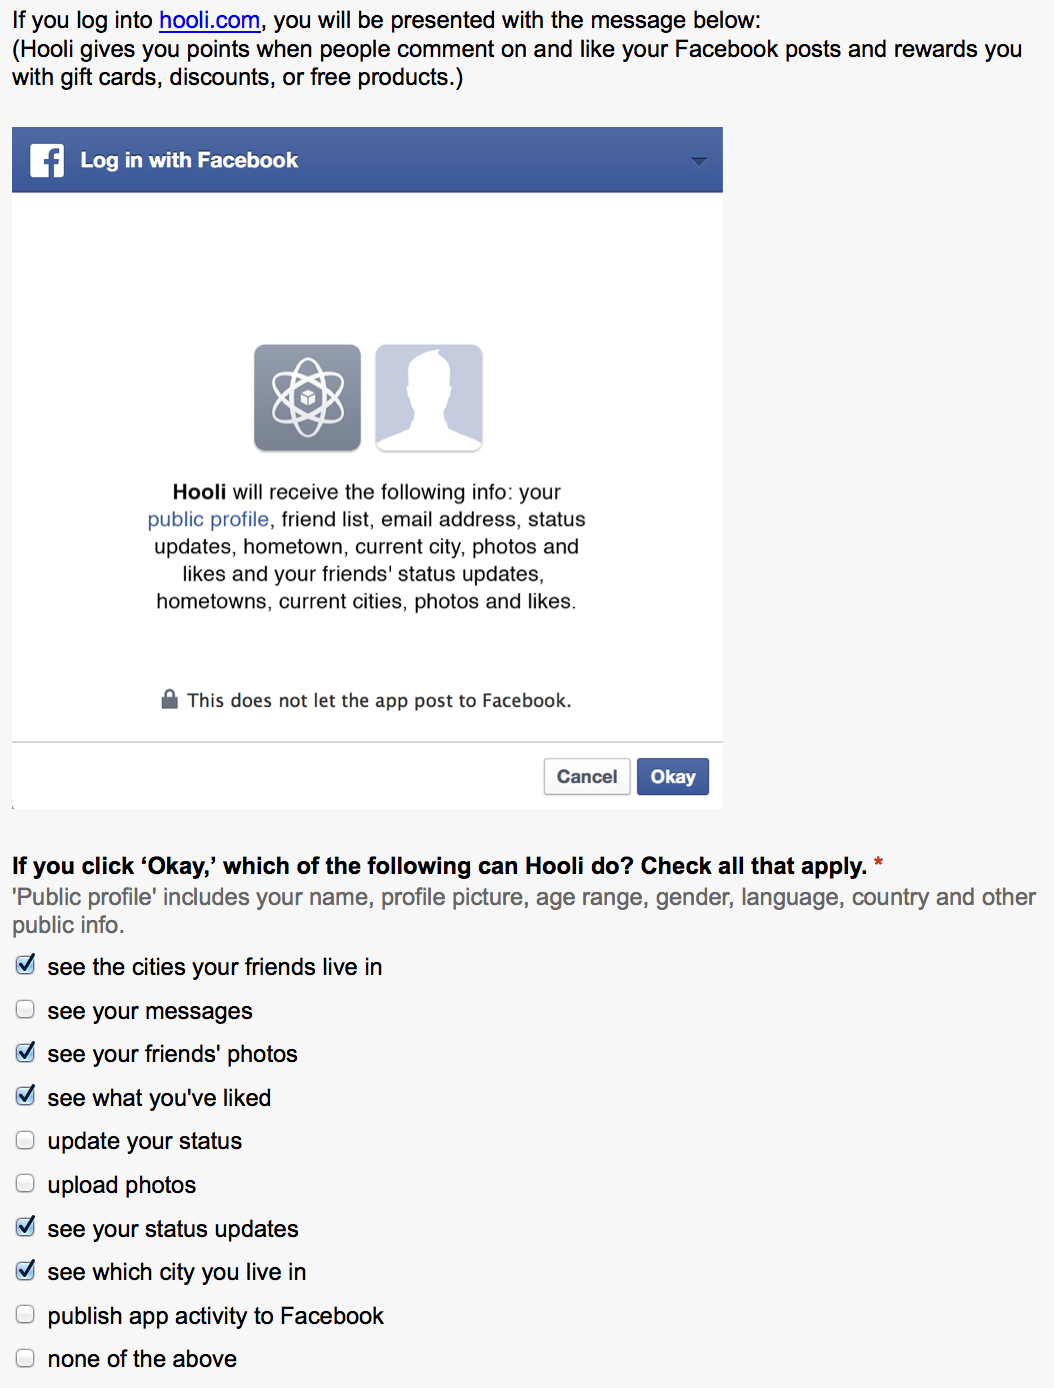
\includegraphics[width=8.5cm]{61r}
  \caption{A read permissions survey. The correct answers are selected. This version of the survey uses the permissions from TripAdvisor.com.}
  \label{figure:61r}
\end{figure}

\begin{figure}[h!]
  \centering
  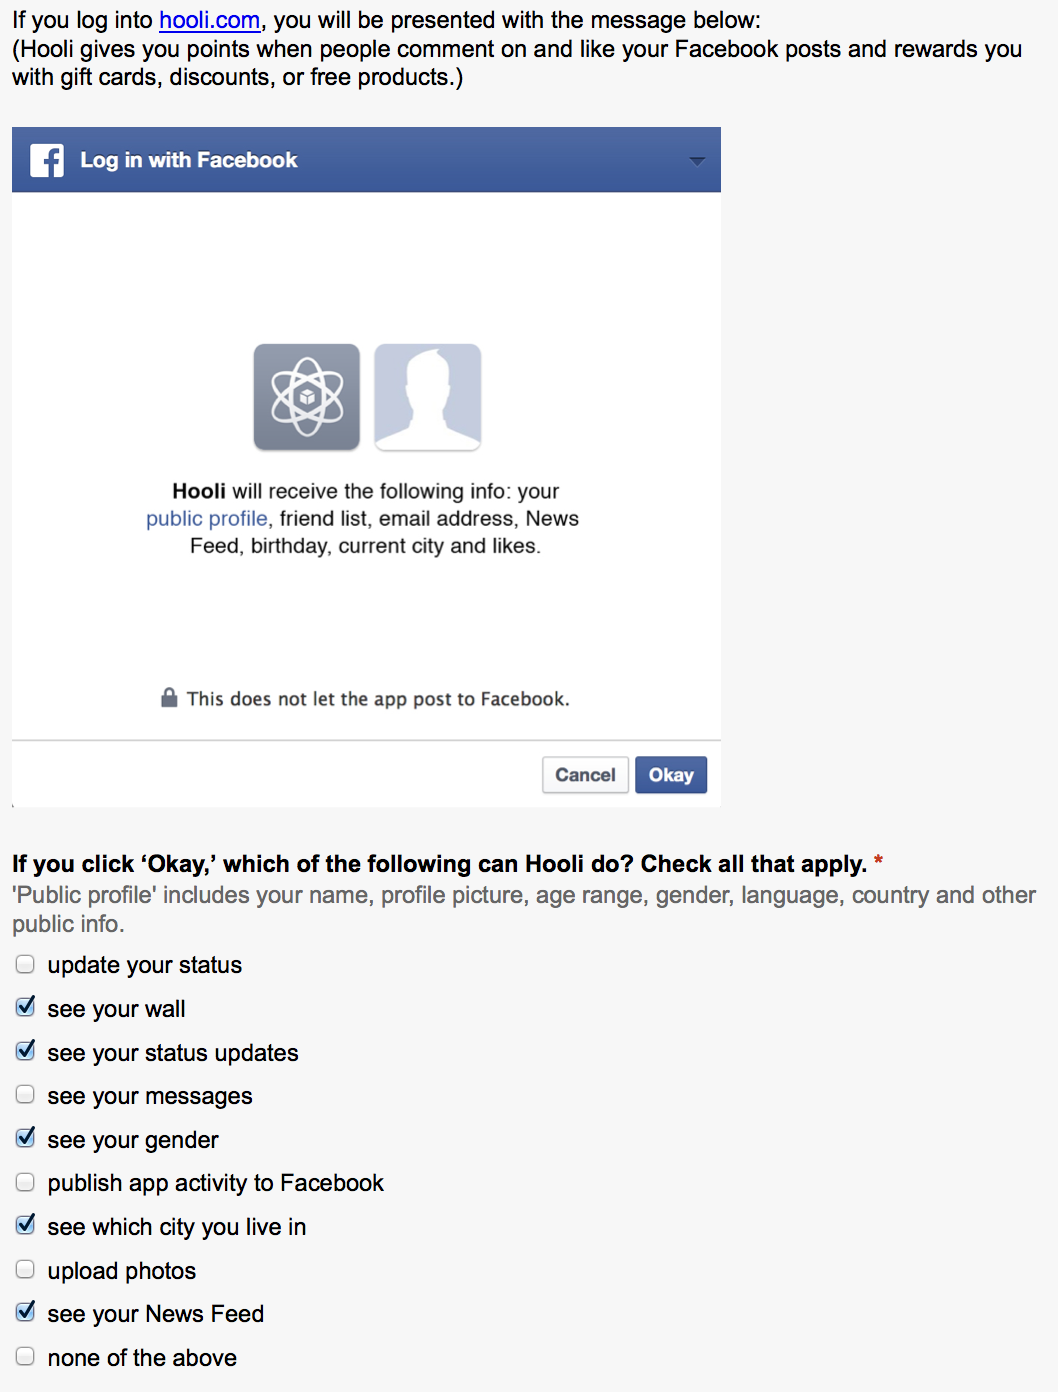
\includegraphics[width=8.5cm]{62r}
  \caption{A read permissions survey. The correct answers are selected. This version of the survey uses the permissions from Splashscore.com.}
  \label{figure:62r}
\end{figure}

\begin{figure}[h!]
  \centering
  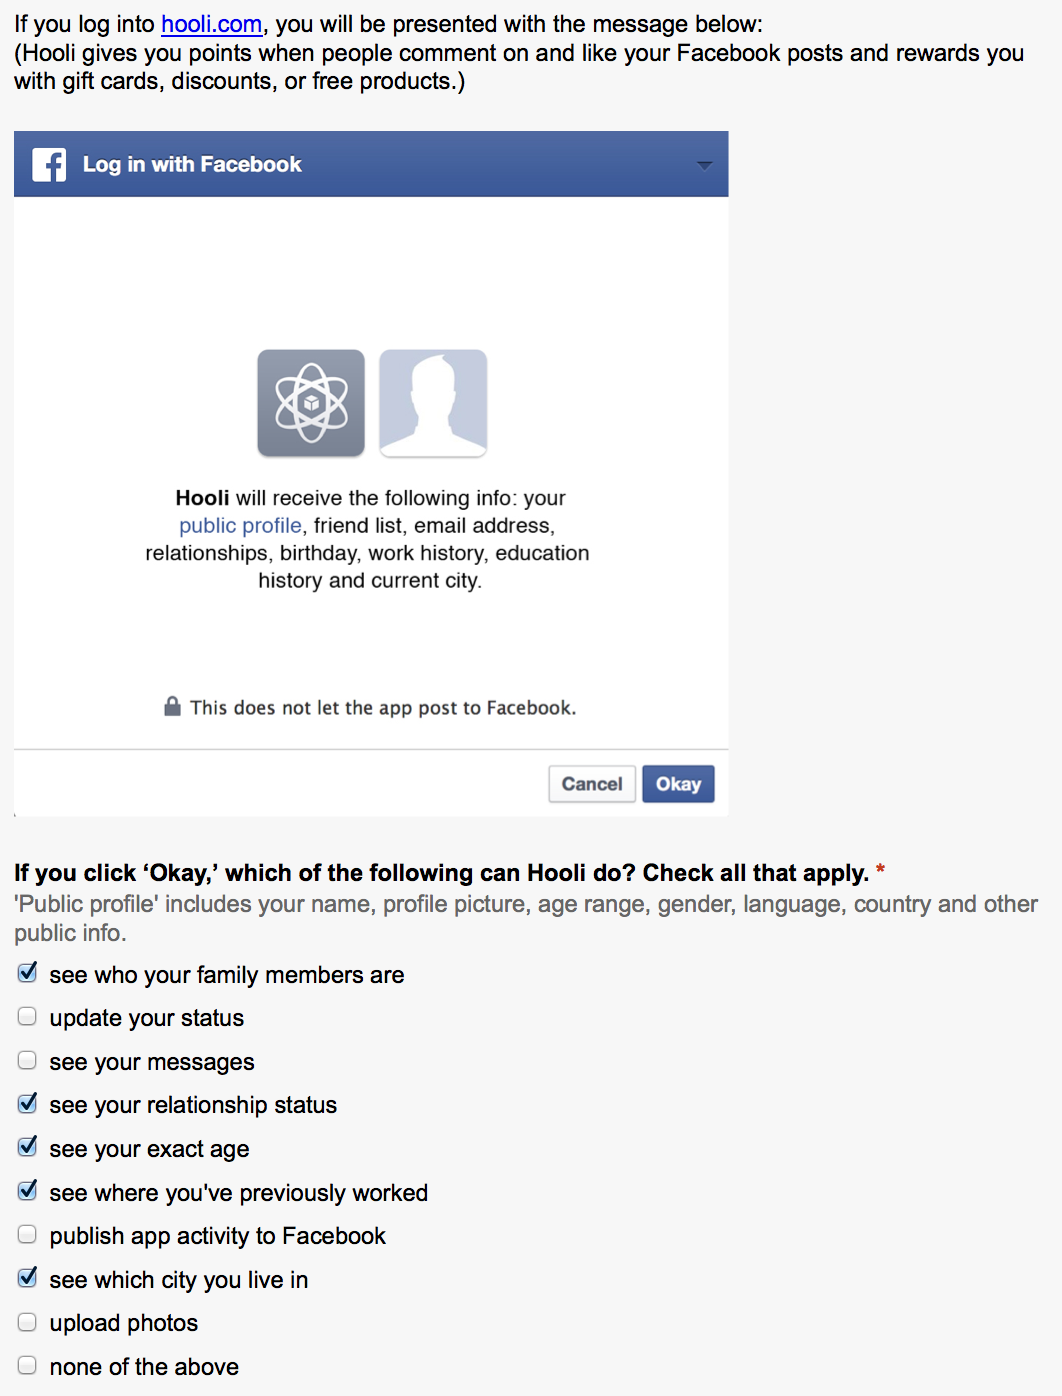
\includegraphics[width=8.5cm]{63r}
  \caption{A read permissions survey. The correct answers are selected. This version of the survey uses the permissions from Jabong.com.}
  \label{figure:63r}
\end{figure}

\begin{figure}[h!]
  \centering
  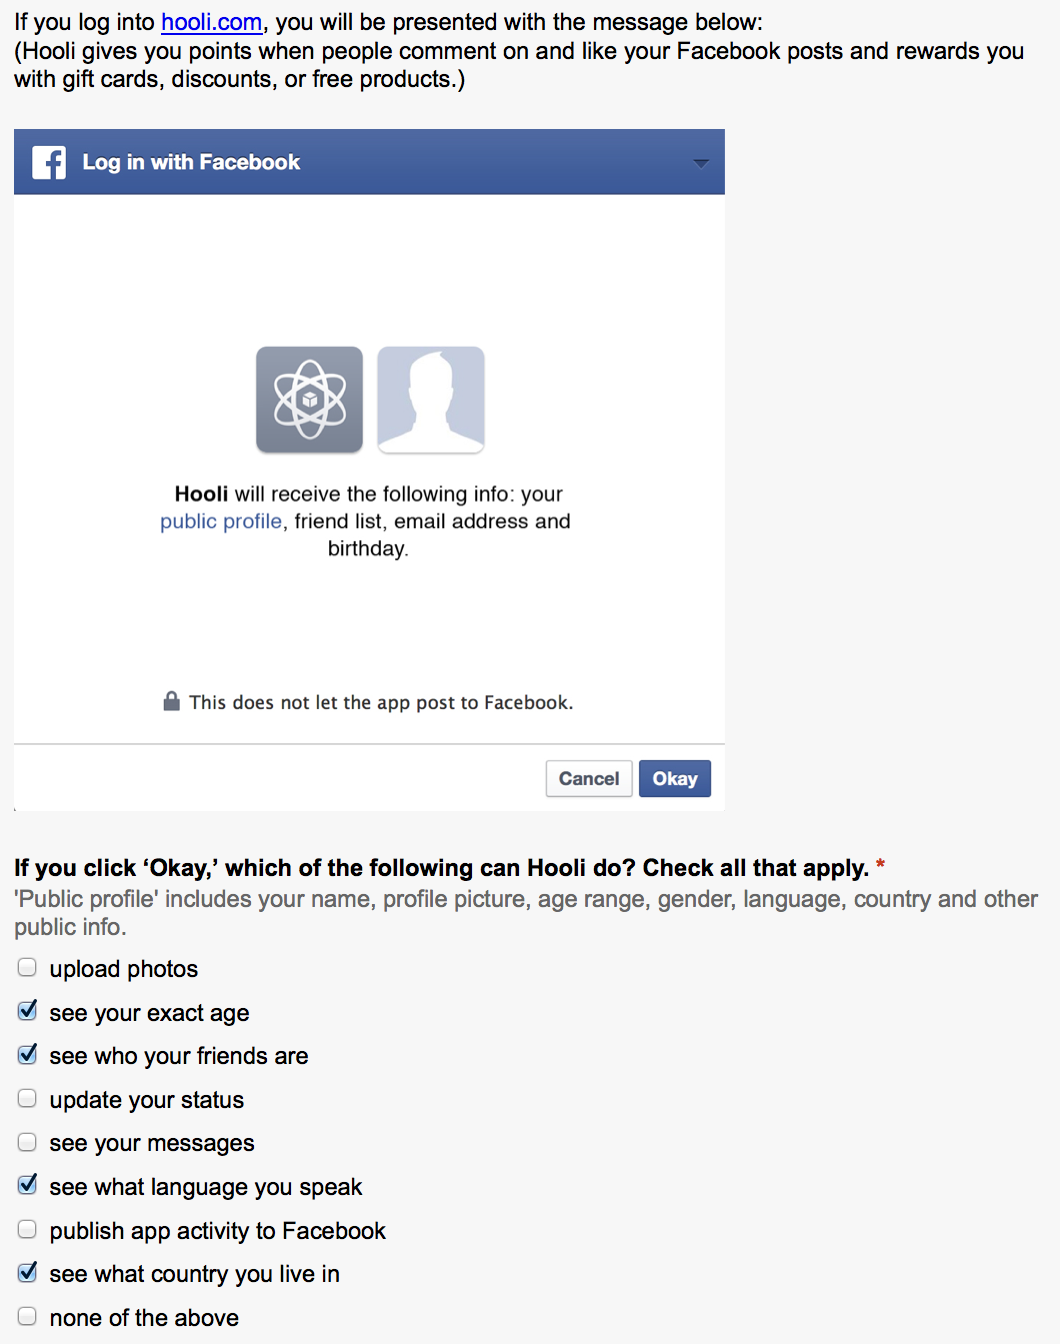
\includegraphics[width=8.5cm]{64r}
  \caption{A read permissions survey. The correct answers are selected. This version of the survey uses the permissions from Flickr.com.}
  \label{figure:64r}
\end{figure}


\subsection{Write permissions surveys}
\label{appendix:writesurveys}

Figure~\ref{figure:61w} shows the survey to test understanding of write permissions. It also uses the fake site ``Hooli.'' The correct answers are selected. There were a total of four versions of this survey with the options in different orders.

\begin{figure}[h!]
  \centering
  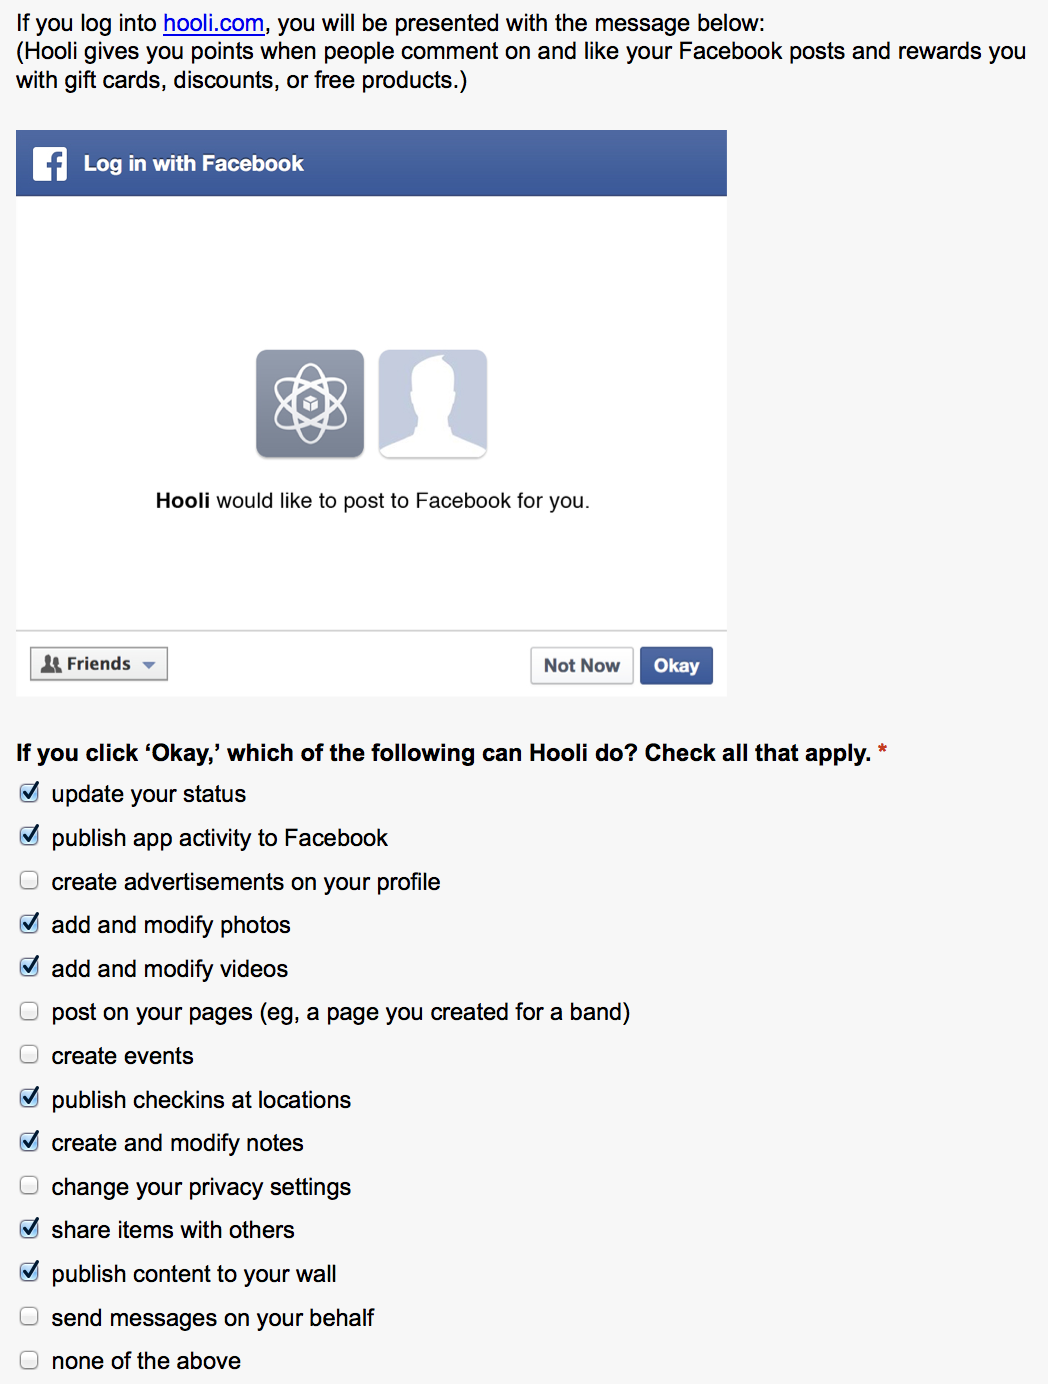
\includegraphics[width=8.5cm]{61w}
  \caption{A write permissions survey. The correct answers are selected.}
  \label{figure:61w}
\end{figure}


\subsection{Additional read permissions survey}
\label{appendix:readsurvey2}
Figure~\ref{figure:71r} shows the survey to test whether users understand that they are giving access to their information that is not marked as visible to the public. The correct answers are selected.

\begin{figure}[h!]
  \centering
  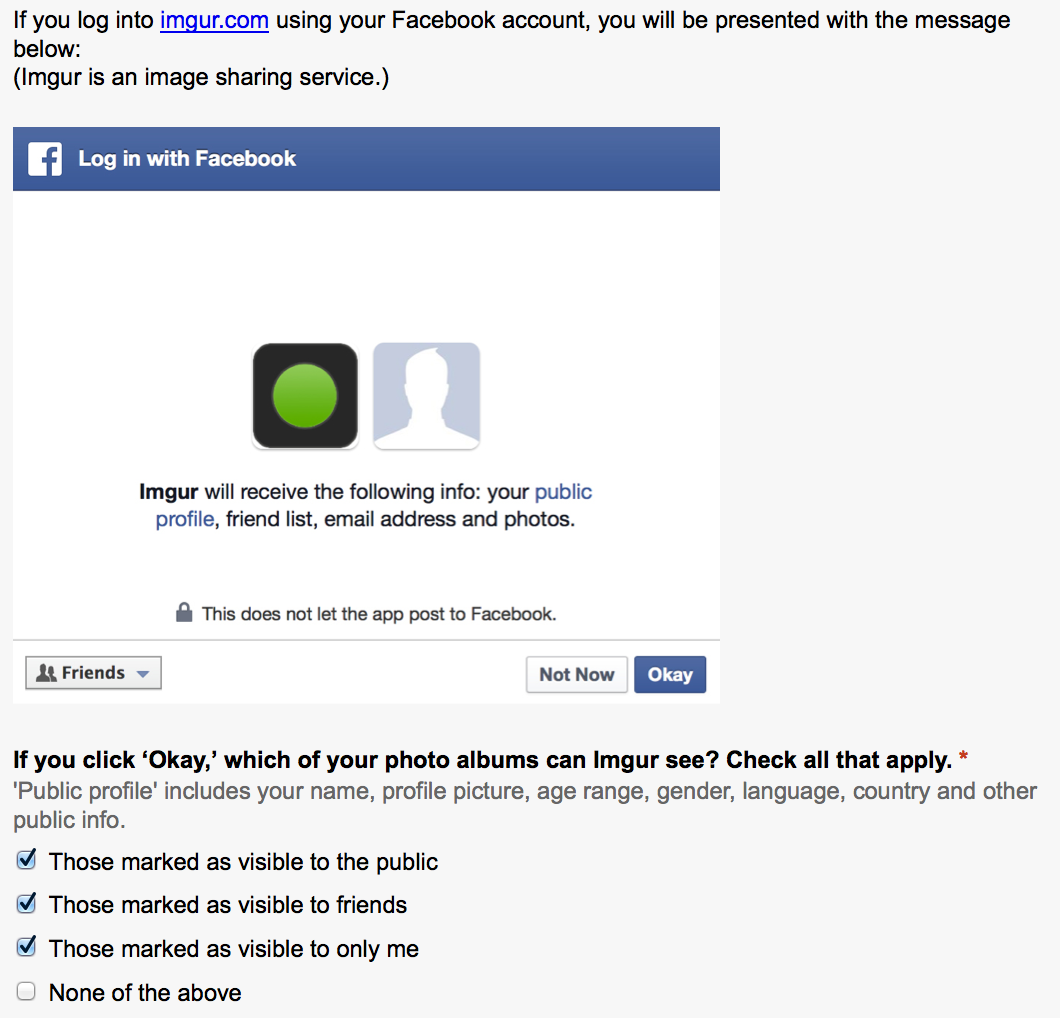
\includegraphics[width=8.5cm]{71r}
  \caption{The additional read permissions survey. The correct answers are selected.}
  \label{figure:71r}
\end{figure}

\FloatBarrier
}{
\clearpage
\appendix
}
\section{Correspondence with Facebook Security}
\label{appendix:correspondence}

As mentioned in Section~\ref{sec:fbresponse}, we sent a security bug report to Facebook reporting that we could use the \emph{publish\_actions} permission after requesting any other write permission (see Section~\ref{sec:developerdiffs}). Below is the full correspondence with Facebook Security \cite{fbsecurity}.

\noindent\rule{6cm}{0.4pt}

\noindent\textbf{Initial bug report}

\noindent \emph{Description and Impact:}

\noindent I can design a site with Facebook Connect that publishes a story with the `publish\_actions' permission. However, if I request any other write/publishing permission, such as `create\_note', I can still use the `publish\_actions' permission and publish the story.  I believe this is a vulnerability because applications may be receiving more capability than they believe they are requesting.

\noindent \emph{Reproduction Instructions / Proof of Concept:}
\begin{enumerate}
  \item I followed the Facebook documentation instructions to create a story with the publish\_actions permission: https://developers.facebook.com/docs/ opengraph/getting-started/
  \item If I replace publish\_actions in data-scope with any other write permission, including create\_note, I can still publish the story. (If I replace it with a read permission such as email I cannot.)
\end{enumerate}

\noindent\rule{6cm}{0.4pt}

\noindent\textbf{Facebook Security's response}

\noindent Thanks for writing in. Can you send in some screenshots of the dialogue you see when requesting the different permissions? I'm curious to see if the wording changes between the two.

\noindent\rule{6cm}{0.4pt}

\noindent\textbf{Our response}

\noindent Below are screenshots of the two messages presented whether I request create\_note or publish\_actions. \textit{[screenshots not shown here, roughly equivalent to Figure~\ref{figure:messageexample}, center image]}

The HTML for these messages has three hidden input elements named read, write, and extended. The permissions requested appear in their value fields. However, if I request any of the 8 write permissions (publish\_actions, publish\_stream, status\_update, video\_upload, photo\_upload, share\_item, create\_note, or publish\_checkins), all 8 appear in the value of the input element named write. I've been researching this for a class project at Princeton University and I've confirmed that this is true on 73 of 73 different websites that request write permissions. The only two write permissions messages between the 73 sites are ``App\_Name would like to post to Facebook for you'' and ``App\_Name would like to post publicly to Facebook for you.'' The presence of ``publicly'' is just determined by the selection on the menu on the bottom left of the message page (second screenshot), not by the permissions being requested.

\noindent\rule{6cm}{0.4pt}

\noindent\textbf{Facebook Security's response}

\noindent I'll confirm with the Platform team, but I believe this is intentional behavior: as you noted, while in the URL you're requesting one scope we actually translate them to a broader set of scopes which are easier for users to understand.

\noindent\rule{6cm}{0.4pt}

\noindent\textbf{Facebook Security's followup}

\noindent I just confirmed with our Platform team that this behavior is by design.

\noindent\rule{6cm}{0.4pt}

\noindent\textbf{Our response}

\noindent Ok, thanks for looking into that. Is there a reason you do that for the write permissions but not for read or extended permissions?

\noindent\rule{6cm}{0.4pt}

\noindent\textbf{Facebook Security's response}

\noindent The Platform team made this change to simplify the experience for developers and for users. My guess would be that generally, write permissions are more similar (ie: creating a note versus creating a video versus posting all are ways to create content on the site that are not very different) whereas read permissions are more distinct (ie: an app which can view your friends does not necessarily need to view your relationships unless major functionality changes).

\noindent \textit{[End of correspondence]}

\end{document}

